% Fucking default pgfsys-dvipdfmx.def screws up normal text, so use another driver
%\def\pgfsysdriver{pgfsys-dvipdfm.def}
\documentclass[10pt, compress, protectframetitle, handout]{beamer}
% handout to deactivate \uncover
% usetitleprogressbar might be needed
%\usepackage{beamerprosper}

% Load BEFORE the theme
\usepackage{ulem}

\usetheme[progressbar=frametitle,block=fill]{metropolis}

\usepackage{pgfpages}
\usepackage{marvosym}
%\usepackage[marvosym]{tikzsymbols}
\usepackage{pgfplots}
\usepackage{tikz}
\usepackage{xifthen}
\usetikzlibrary{quotes,angles}
\usetikzlibrary{arrows}
\usetikzlibrary{calc,decorations.markings}
\usetikzlibrary{patterns}
\definecolor{myred}{rgb}{0.7,0.1,0.1}
\definecolor{myblue}{rgb}{0,0.447,0.741}
\definecolor{mygreen}{rgb}{0,0.498,0}
\definecolor{silvergray}{rgb}{0.752941176,0.752941176,0.752941176}
\setbeamertemplate{note page}[plain]
%\setbeameroption{show notes on second screen=right}

\usepackage{multirow}
\usepackage{multicol}
\usepackage{booktabs}
\usepackage{adjustbox}

\usepackage{datetime}
%	\usepackage[scale=2]{ccicons}
%	\usepackage{minted}
%	\usepgfplotslibrary{dateplot}
%	\usemintedstyle{trac}

\usepackage{textpos}
% Fixes bad positioning of hats
\usefonttheme{professionalfonts}%[onlymath]{serif}
\usepackage{subcaption}
%\usepackage{epstopdf}
\usepackage{siunitx}
\DeclareSIUnit\atomicunit{a.u.}
\DeclareSIUnit\rydberg{Ry}
\usepackage{braket}
\usepackage{comment}
\usepackage{cancel}
%\includecomment{versionLONG}
\excludecomment{versionLONG}
\usepackage[sort&compress,square,semicolon]{natbib}

\def\qe{{\textsc Quantum ESPRESSO}}
\newcommand{\MATLAB}{MATLAB\textsuperscript{\textregistered}}

% Declare porous pattern
\pgfdeclarepatternformonly{porous}{\pgfqpoint{-2pt}{-2pt}}{\pgfqpoint{7.5pt}{7.5pt}}{\pgfqpoint{6.4pt}{5pt}}%
{
	\pgfpathcircle{\pgfqpoint{0pt}{1.2pt}}{1.5pt}
	\pgfpathcircle{\pgfqpoint{3.2pt}{3.7pt}}{1.5pt}
	\pgfusepath{fill}
}

%%%%%%%%%%%%%%%%%%%%%%%%%%%%%%%%%%%%%%%%%%%%%%%%%%%%%%%%%%%
% datetime specific configuration                         %
%%%%%%%%%%%%%%%%%%%%%%%%%%%%%%%%%%%%%%%%%%%%%%%%%%%%%%%%%%%
\newdateformat{monthyear}{\monthname[\THEMONTH] \THEYEAR}

\graphicspath{{figures/PNG/}{figures/PDF/}{figures/}}

%\addtobeamertemplate{frametitle}{}{%
%\begin{textblock*}{1.5cm}(-0.7cm,0.7\textheight)
%\includegraphics[height=1.5cm]{logo_unitn}
%\end{textblock*}}

\title{Simulation of the Lennard-Jones fluid in the NVT ensemble}
\subtitle{A presentation for the course in \emph{Computer Simulation}}
\date{December 27, 2016}
\author{Matteo Seclì}
\institute{\scshape SISSA - Doctorate School in Condensed Matter
\vfill
\hfill\includegraphics[height=1.3cm]{SISSA-LOGO.pdf}}
%\titlegraphic{\hfill\includegraphics[height=1.3cm]{SISSA-LOGO.pdf}}

\addtobeamertemplate{frametitle}{}{%
\begin{textblock*}{100mm}(0.96\textwidth,-0.9cm)
\includegraphics[height=0.8cm]{sissa_logo_white.png}
\end{textblock*}}

\begin{document}

\maketitle

\begin{frame}{Contents}
	\tableofcontents
\end{frame}


\section{Introduction}

\begin{frame}{Implementation choices}
	
	\begin{figure}
		\centering
		\includegraphics[height=0.25\textwidth]{Cpp_logo}
		$\qquad$
		\includegraphics[height=0.15\textwidth]{armadillo_logo}
		$\qquad$
		\includegraphics[height=0.25\textwidth]{QtCreator}
		\bigskip\medskip\linebreak
		\includegraphics[height=0.25\textwidth]{matlab_logo}
		$\qquad\qquad$
		\includegraphics[height=0.25\textwidth]{github_logo}
	\end{figure}

	Code at: \url{https://github.com/matteosecli/LJMC}.	
	
\end{frame}


\section{Simulation background}

\begin{frame}{The system}
	
	\begin{figure}
		\centering
		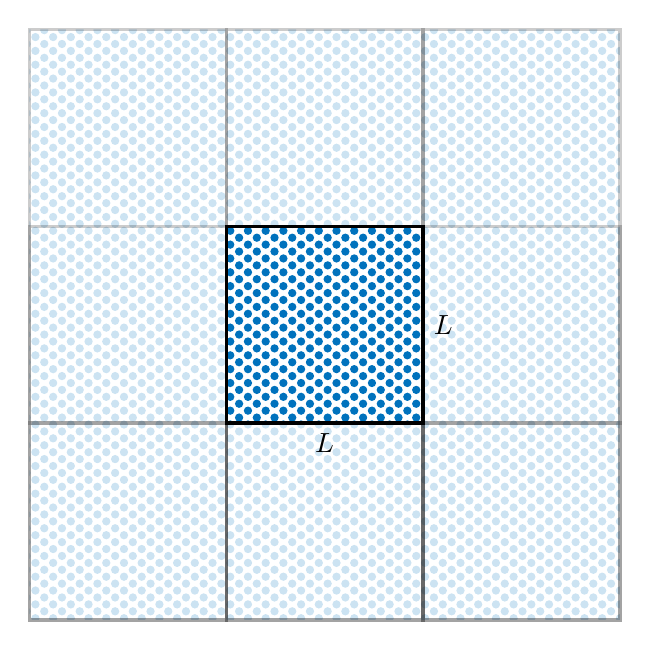
\begin{tikzpicture}[>=latex,transform shape,scale=1.0]
			% Set the lengths of the system
			\pgfmathsetmacro{\L}{2.5};
			
			% Draw a filling
			%\begin{scope}
			%	\clip (-\L/2,-\L/2) rectangle (\L/2,\L/2);
			%	\filldraw[color=myblue] (0,0) circle (0.1);
			%\end{scope}
			
			% Draw the porous pattern
			\fill [pattern=porous, pattern color=myblue, opacity=0.2, even odd rule] (-\L*1.5,-\L*1.5) rectangle (\L*1.5,\L*1.5) -- (-\L/2,-\L/2) rectangle (\L/2,\L/2);
			\fill [pattern=porous, pattern color=myblue] (-\L/2,-\L/2) rectangle (\L/2,\L/2);
			
			% Draw other light boxes
			\draw[very thick, opacity=0.2] (-\L*1.5,-\L*1.5) rectangle (-\L*0.5,-\L*0.5);
			\draw[very thick, opacity=0.2] (-\L*1.5,-\L*0.5) rectangle (-\L*0.5,\L*0.5);
			\draw[very thick, opacity=0.2] (-\L*1.5,-\L*1.5) rectangle (-\L*0.5,\L*1.5);
			\draw[very thick, opacity=0.2] (-\L*0.5,-\L*1.5) rectangle (\L*0.5,-\L*0.5);
			% The box in this point is already there
			\draw[very thick, opacity=0.2] (-\L*0.5,-\L*1.5) rectangle (\L*0.5,\L*1.5);
			\draw[very thick, opacity=0.2] (\L*0.5,-\L*1.5) rectangle (\L*1.5,-\L*0.5);
			\draw[very thick, opacity=0.2] (\L*0.5,-\L*0.5) rectangle (\L*1.5,\L*0.5);
			\draw[very thick, opacity=0.2] (\L*0.5,-\L*1.5) rectangle (\L*1.5,\L*1.5);

			% Draw the main box
			\draw[very thick] (-\L/2,-\L/2) -- (\L/2,-\L/2) node[midway,below] {$L$} 
				-- (\L/2,\L/2) node[midway,right] {$L$}-- (-\L/2,\L/2) -- cycle;
		\end{tikzpicture}
	\end{figure}	
	
\end{frame}

\begin{frame}[allowframebreaks]{The system -- remarks}
	
	\begin{itemize}
		\item The system is 3D, but the best I can sketch is a 2D system. Sorry about that.
		\item We want to do (macroscopic) thermodynamics ($\sim N_A$ particles), but today's computers can handle at most a few thousand particles. One can usually do two things:
		\begin{itemize}
			\item do the calculations in a \alert{finite box} containing a \alert{finite number} of particles, and then take the thermodynamic limit;
			\item do the calculations in a \alert{finite box} containing a \alert{finite number} of particles, but with \alert{periodic boundary conditions} (that make the system artificially infinite).
		\end{itemize}
		\item The problem with the first way is that for small systems (as the ones we can simulate) the choice of boundary conditions could have a non-negligible effect on the properties of the system (\cite{Frenkel2002}). An an example, for a 3D sc crystal with 1000 atoms and free boundaries, $\SI{49}{\percent}$ of all the atoms is on the surface. This means that our simulated system would be plagued by surface effects that we don't wont, since we are interested in \alert{bulk properties}.
		\item The choice of PBC's is therefore not casual, since they mimic the presence of an infinite bulk surrounding the region (i.e., the box) we are studying. Beware that this model is not anyway exempt from size effects, since in the end we are trying to get the properties of a thermodynamical system by assuming that it can be described by ``gluing'' \alert{identical copies} of a non-thermodynamical system.
	\end{itemize}
	
\end{frame}

\begin{frame}[allowframebreaks]{The potential}

	The pair potential is assumed to be of Lennard-Jones type (see Figure \ref{fig:LJ}).
	
	Typical expressions are:
	\begin{equation}
		v_{\mathrm{LJ}}(r) = 4\varepsilon\left[\left(\frac{\sigma}{r}\right)^{12}-\left(\frac{\sigma}{r}\right)^{6}\right]
	\end{equation}
	or equivalently
	\begin{equation}
		v_{\mathrm{LJ}}(r) = \varepsilon\left[\left(\frac{r_{\min}}{r}\right)^{12}-2\left(\frac{r_{\min}}{r}\right)^{6}\right],
	\end{equation}
	where $r_{\min} = 2^{1/6}\sigma$.
	
	\begin{figure}
		\begin{tikzpicture}[>=latex,transform shape,scale=1.0]
			% Draw axes
			\draw[->] (2.50,0) -- (10,0) node[right] {$r$};
    		\draw[->] (2.70,-1.5) -- (2.70,4) node[above] {$v_{\mathrm{LJ}}(r)$};
    		
    		% Draw the LJ potential
			\draw[thick,domain=0.93:3,smooth,samples=400,variable=\r,color=myblue,xscale=3] plot[id=LJ] ({\r},{4*( (1/\r)^12 - (1/\r)^6 )});
			
			% Draw some references
			\draw[dashed] (2.70,-1) node[left] {$-\varepsilon$} -- (3.367,-1);
			\draw[dashed] (3.367,0) node[above] {$r_{\min}$} -- (3.367,-1);
		\end{tikzpicture}
		\caption{The Lennard-Jones potential.}
		\label{fig:LJ}
	\end{figure}

\end{frame}

\begin{frame}[allowframebreaks]{Cutoff: why, when, where, how}

	As you see, the potential we are using is defined in the whole interval $r \in (0,\infty)$. Thus, in principle it allows interactions between an atom $i$ and all the other atoms in the box (except $i$ itself) plus all their images in the mirror boxes. It's an \alert{infinite} number of interactions!
	
	However you see that for large distances the pair interaction is small compared to $\varepsilon$, so it seems reasonable to make interact atom $i$ only with all the other atoms that fall within a certain distance from it. This distance is called the \alert{cutoff radius $r_c$}. Mathematically, the whole deal is to redefine the potential as
	\begin{equation}
		v_{\mathrm{LJ}}^{\text{trunc}}(r) =
		\begin{cases}
			v_{\mathrm{LJ}} & r \leq r_c \\
			0 & r > r_c
		\end{cases}
	\end{equation}
	
	The part of the potential we are discarding by doing this approximation can be re-added back through a correction (per particle) that reads as (\cite{Frenkel2002})
	\begin{equation}
		v_{\mathrm{LJ}}^{\text{tail}}(r_c) = \frac{1}{2}\int_{r_c}^{\infty}d\vec{r}\,\rho(r)v_{\mathrm{LJ}}(r),
	\end{equation}
	where $\rho(r)$ can be rewritten as $\rho(r) = \rho g(r)$. Since one doesn't know the density in advance (and thus cannot solve the integral), the cutoff radius $r_c$ is chosen in such a way that from there on the density $\rho(r)$ is approximately equal to its uniform value $\rho$, i.e. $g(r)=1$. With this caveat in mind, the integral is easily solvable and our calculations can be done with a new pair potential defined as
	\begin{equation}
		v_{\mathrm{LJ}}^{\text{trunc}}(r) + v_{\mathrm{LJ}}^{\text{tail}}(r_c) \approx v_{LJ}(r).
	\end{equation}
	The goodness of this approximation depends on the choice of $r_c$, and it becomes exact in the limit $r_c \to \infty$.
	
\end{frame}

\begin{frame}{Importance of tail corrections}

	As an example, $v_{LJ}(r_c=2.5\sigma) = \varepsilon/60$. It could then seem that the tail correction is negligible, but if you do the explicit calculation you realize that it's actually around $\SI{10}{\percent}$ of the potential energy per atom (\cite{Frenkel2002}). Therefore, the tail correction is quite relevant.
	
	However, if the cutoff radius is not large enough the tail correction could then under- or over-estimate the real potential, because the approximation $g(r)$ is not good anymore. A correct choice for the cutoff radius requires a bit of experimentation: first you run the simulation and you calculate the $g(r)$, and then if you see that at $r_c$ the $g(r)$ cannot be safely approximated with $1$, you increase the $r_c$.
	
	The tail corrections are even more relevant when it comes to the pressure, but let's first say a few words about it.

\end{frame}

\begin{frame}[allowframebreaks]{Calculation of the pressure}

	The pressure of the system can be obtained from the \alert{virial theorem}, which is a sort of ``generalized equipartition'' theorem. For a set of generalized coordinates $\{q_k\}$ and their conjugate momenta $\{p_k\}$, the theorem can be stated as (see \cite{Galli})
	\begin{equation}
		\Braket{p_k\frac{\partial H}{\partial p_k}} = \Braket{q_k\frac{\partial H}{\partial q_k}} = k_BT.
	\end{equation}
	
	From the second equality, it takes a few lines to show that
	\begin{equation}
		P = \rho k_B T + \frac{\Braket{W}}{V},
	\end{equation}
	where
	\begin{equation}
		\Braket{W} = \frac{1}{3} \sum_{i=1}^{N} \vec{r}_{i} \cdot \vec{f}_{i} 
	\end{equation}
	is called the \alert{virial}.
	
	Because of the truncation of the potential, one can define a tail correction for the pressure as before:
	\begin{equation}
		P^{\text{tail}} = \frac{1}{V}\frac{1}{3}N\frac{1}{2}\int_{r_c}^{\infty}d\vec{r}\,\rho(r) \vec{r} \cdot \vec{f}(r) \approx -\frac{1}{6}\rho^2\int_{r_c}^{\infty}dr\,4\pi r^3\frac{\partial v_{LJ}(r)}{\partial r}.
	\end{equation}
	where $1/3$ comes from the definition of the virial, $1/2$ is there to avoid the double counting of the interactions (as for the potential), and $N$ is there because this is the \emph{total} pressure, so we have to multiply the correction on the pair-potential by the total number of particles. Again, we've approximated $g(r)$ to $1$ so that the integral can be easily found via integration by parts.
	
	In principle, the true correction would have been an \emph{impulsive} correction to the pressure, coming from the jump discontinuity of the pair-potential at $r_c$. However, the \emph{real} potential is \emph{not} discontinuous; the truncation is just a trick to handle the calculation, it has no physical meaning. Therefore, the impulsive correction is not usually included. If instead the true potential was really discontinuous, then the impulsive correction should have been included instead of the tail correction.

\end{frame}

\begin{frame}[allowframebreaks]{Choice of $r_c$ in our system}
	
	To make the computation easy, we decided to set $r_c=L/2$, as shown in Figure \ref{fig:fluid_cutoff}.
	
	\begin{figure}
		\centering
		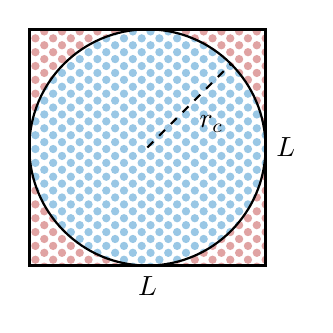
\begin{tikzpicture}[>=latex, transform shape, scale=1.0]
			% Set the lengths of the system
			\pgfmathsetmacro{\L}{3};
			% Draw the porous pattern
			\fill [pattern=porous, pattern color=myred, opacity=0.4, even odd rule] (-\L/2,-\L/2) rectangle (\L/2,\L/2) -- (0,0) circle (\L/2);
			\fill [pattern=porous, pattern color=myblue, opacity=0.4] (0,0) circle (\L/2);
			
			% Draw the main box
			\draw[very thick] (-\L/2,-\L/2) -- (\L/2,-\L/2) node[midway,below] {$L$} 
				-- (\L/2,\L/2) node[midway,right] {$L$}-- (-\L/2,\L/2) -- cycle;
				
			% Draw the cutoff circle and the cutoff radius
			\draw[thick] (0,0) circle (\L/2);
			\draw[dashed, thick] (0,0) -- ({\L*sqrt(2)*0.5*0.5},{\L*sqrt(2)*0.5*0.5}) node[midway, below right] {$r_c$};
		\end{tikzpicture}
		\caption{Visual scheme of the cutoff. The central atom interacts with the blue ones, within a circle of radius $r_c$, while the interactions with the red atoms are discarded.}
		\label{fig:fluid_cutoff}
	\end{figure}
	
	Beware that, since $r_c$ depends on $L$, this is a choice that \alert{depends on the number of atoms} used in the simulation -- at fixed density. Therefore, this choice must be carefully balanced with a correct choice of the number of particles.
	
	As an example, let's suppose we are simulating $N=100$ particles with density $\rho = 0.9$ and temperature $T=0.9$ (if not differently specified, all quantities are given in \alert{reduced units}). This choice is equivalent to the choice $r_c \simeq 2.40$; let's look at the radial distribution function at this value:
	
	\begin{figure}
		\includegraphics[width=\textwidth]{g(r)_N100}
		\caption{$g(r)$ for $N=100$ atoms, at $\rho=0.9$ and $T=0.9$.}
	\end{figure}
	
	The simulation results are: $\Braket{V}/N = -6.23 \pm 0.01$, $\Braket{P} = 2.34 \pm 0.03$. The tail corrections amount to $\SI{9}{\percent}$ of the final value of the potential and to $\SI{42}{\percent}$ of the final value of the pressure.
	
	As you see, such a choice is a bit rough: our tail corrections will probably not be faithful since the $g(r)$ cannot be safely approximated to $1$ at $r_c$. Furthermore, since $g(r_c) < 1$, we are getting a value for the energy which is lower than the exact one; a better choice of the cutoff will give a higher value of the energy, which is more near to the correct one.
	
	The right approach to this problem is to choose in advance a value for the cutoff radius; let's choose for example $r_c=3.0$, which means $L=6$. For such a box, the number of atoms required to simulate a system with density $\rho=0.9$ is roughly $194$. Let's do again the simulation and look at the result:
	
	\begin{figure}
		\includegraphics[width=\textwidth]{g(r)_N194}
		\caption{$g(r)$ for $N=194$ atoms, at $\rho=0.9$ and $T=0.9$.}
	\end{figure}
	
	The simulation results are: $\Braket{V}/N = -6.180 \pm 0.003$, $\Braket{P} = 2.55 \pm 0.02$. The tail corrections amount to $\SI{5}{\percent}$ of the final value of the potential and to $\SI{20}{\percent}$ of the final value of the pressure: we've reduced them by a half! As predicted, the value of the potential is also slightly higher and more near to the actual value.
	
	You can also push it further and simulate $N=500$ atoms, which for $\rho=0.9$ correspond to $r_c \simeq 4.1$.
	
	\begin{figure}
		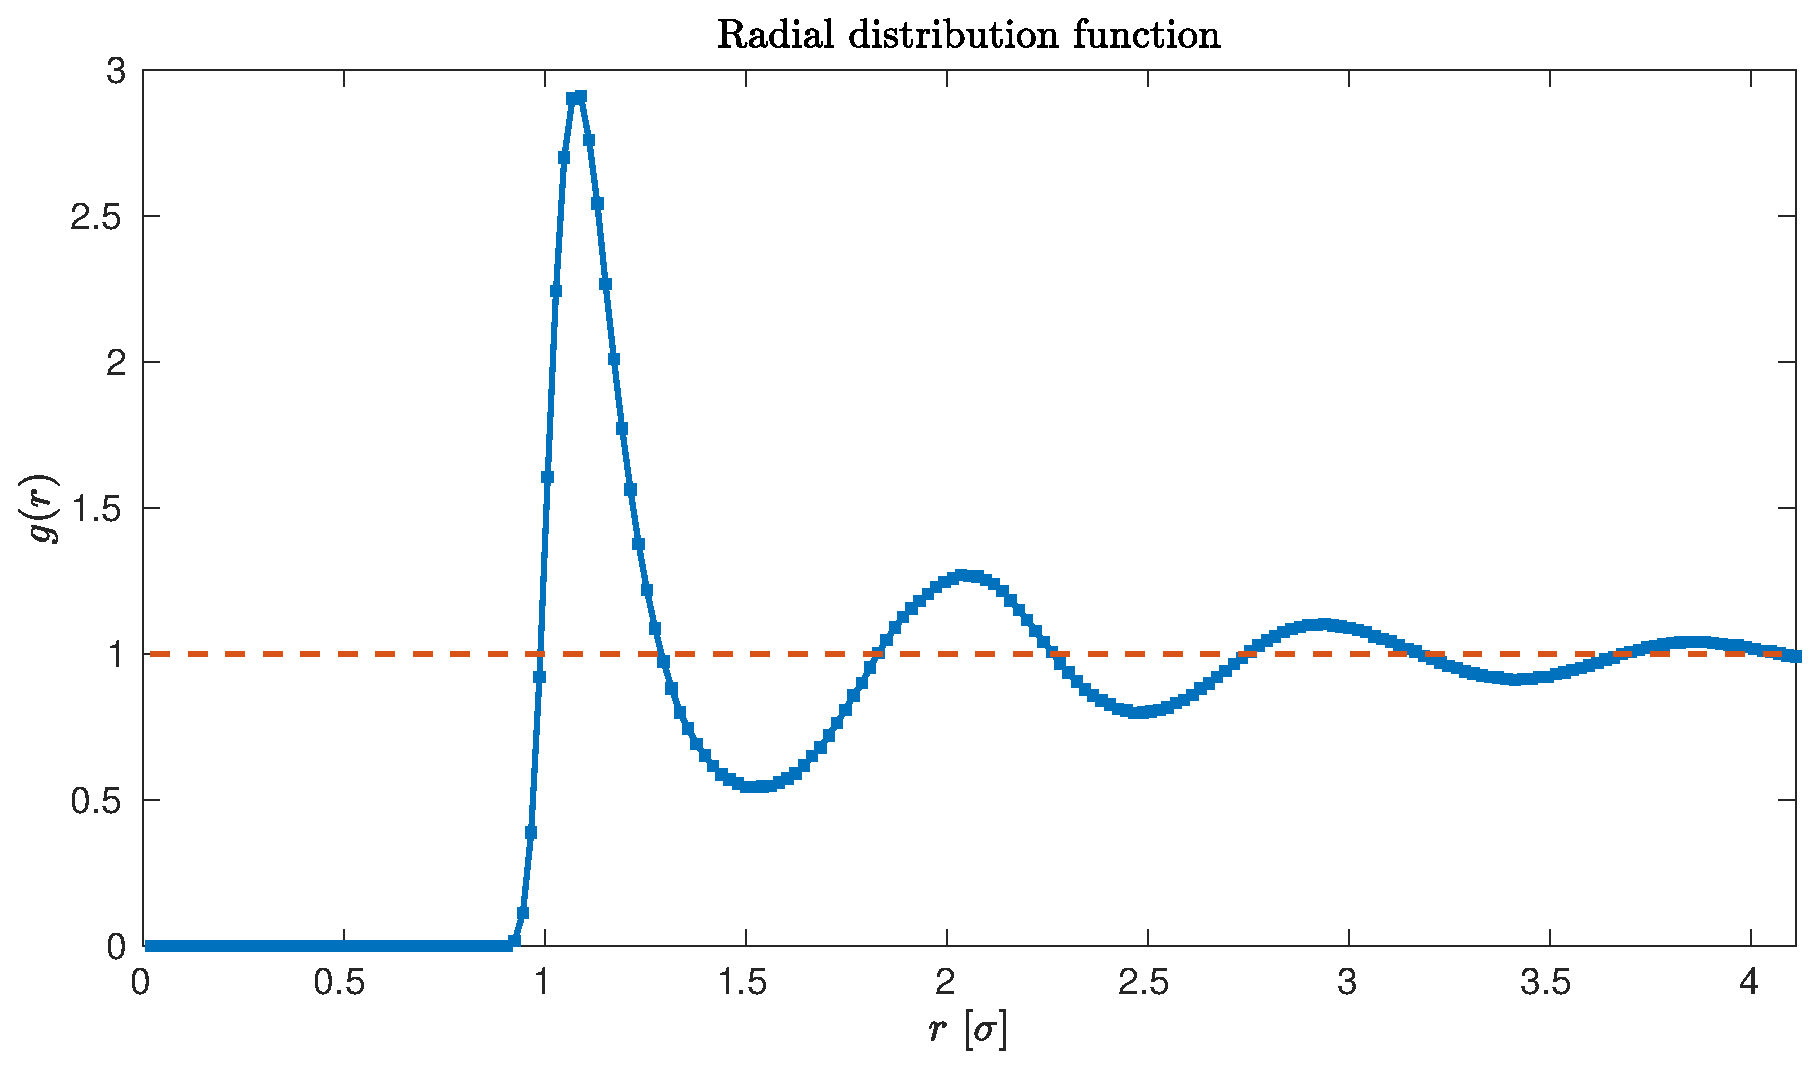
\includegraphics[width=\textwidth]{g(r)_N500}
		\caption{$g(r)$ for $N=500$ atoms, at $\rho=0.9$ and $T=0.9$.}
	\end{figure}
	
	The simulation results are: $\Braket{V}/N = -6.174 \pm 0.005$, $\Braket{P} = 2.55 \pm 0.03$. The tail corrections amount to $\SI{2}{\percent}$ of the final value of the potential and to $\SI{8}{\percent}$ of the final value of the pressure.
	
	As you see such a choice is a bit an \alert{overkill} for many purposes, because the results are compatible within an error bar and we've gained nothing in precision. Moreover, this was at the expenses of the computational time; since the algorithm scales as the square of the number of particles, the $N=500$ case takes roughly $6.6$ times more than the $N=194$ case.
	
\end{frame}

\begin{frame}[allowframebreaks]{Other technical details}
	\begin{itemize}
		\item \underline{Initialization.} The result of the simulation, for a certain set of parameters, must be the same \alert{no matter what is the initial arrangement of the atoms}. However, due to numerical errors, it's better not to initialize the potential to values that are near (or beyond, of course) the machine precision. In the present case, we have to avoid the situation in which, due to a random initialization of the positions, two or more atoms come so close that the corresponding potential term goes to infinity (at least, compared to the machine precision). The simplest way to avoid this situation is to initialize the atoms in a uniform ``lattice'' contained in the box, as shown in Figure \ref{fig:initialization_scheme}. Briefly, we simply calculate the minimum square $n^2$ (for the 2D case, or the minimum cube for the 3D case) that is greater or equal to the given number of atoms, and then fill an imaginary lattice which has $n$ atoms per side.
		\begin{figure}
			\centering
			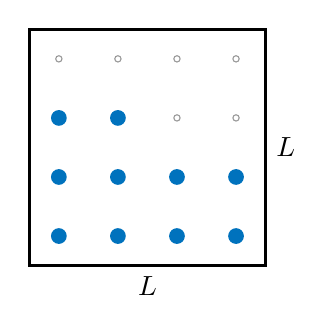
\begin{tikzpicture}[>=latex, transform shape, scale=1.0]
				% Set the lengths of the system
				\pgfmathsetmacro{\L}{3};
				\pgfmathsetmacro{\dL}{\L/8};
				
				% Draw the main box
				\draw[very thick] (-\L/2,-\L/2) -- (\L/2,-\L/2) node[midway,below] {$L$} 
					-- (\L/2,\L/2) node[midway,right] {$L$}-- (-\L/2,\L/2) -- cycle;
					
				% Put 10 atoms in the imaginary lattice, 4x4.
				%\fill[myblue] (0,0) circle (0.1);
				\foreach \j in {0,...,3}
				{
					\foreach \i in {0,...,3}
					{
						\pgfmathtruncatemacro{\nP}{4*\j+\i+1};
						\ifthenelse{\NOT \nP > 10}{\fill[myblue] ({-\L/2+(2*\i+1)*\dL},{-\L/2+(2*\j+1)*\dL}) circle (0.1);}{\draw[black!40!white] ({-\L/2+(2*\i+1)*\dL},{-\L/2+(2*\j+1)*\dL}) circle (0.04);}
					}
				}
			\end{tikzpicture}
			\caption{Schematic initialization of $10$ particles in a 2D box. The grey circles are the ``empty lattice sites'' that exceed the given number of particles.}
			\label{fig:initialization_scheme}
		\end{figure}
		\item \underline{Treatment of the uncertainties.} The uncertainties have been calculated with the \alert{binning technique}.
		\begin{itemize}
			\item The idea is to divide the dataset into $M$ bins, each one with $L$ samples, such that $M \times L$ is the total number of samples.
			\item Then you build the set of the means $\{\Braket{V}_m\}$, $m \in 1,\ldots,M$, of which you calculate the standard deviation $\sigma_M$.
			\item At this point, the uncertainty on the mean $\Braket{V}$ of the whole sample can be estimated as $\sigma_M/\sqrt{M}$.
			\item Then, you repeat this procedure for different values of $M$ (and thus of $L$) and you plot $\sigma_M/\sqrt{M}$ vs $L$.
			\item At a certain point, the uncertainty should reach a \alert{plateau} value, that you take as the final estimator of the uncertainty of $\Braket{V}$.
		\end{itemize}
		A typical result of this procedure is shown in Figure \ref{fig:binning_example}.
		\begin{figure}
			\centering
			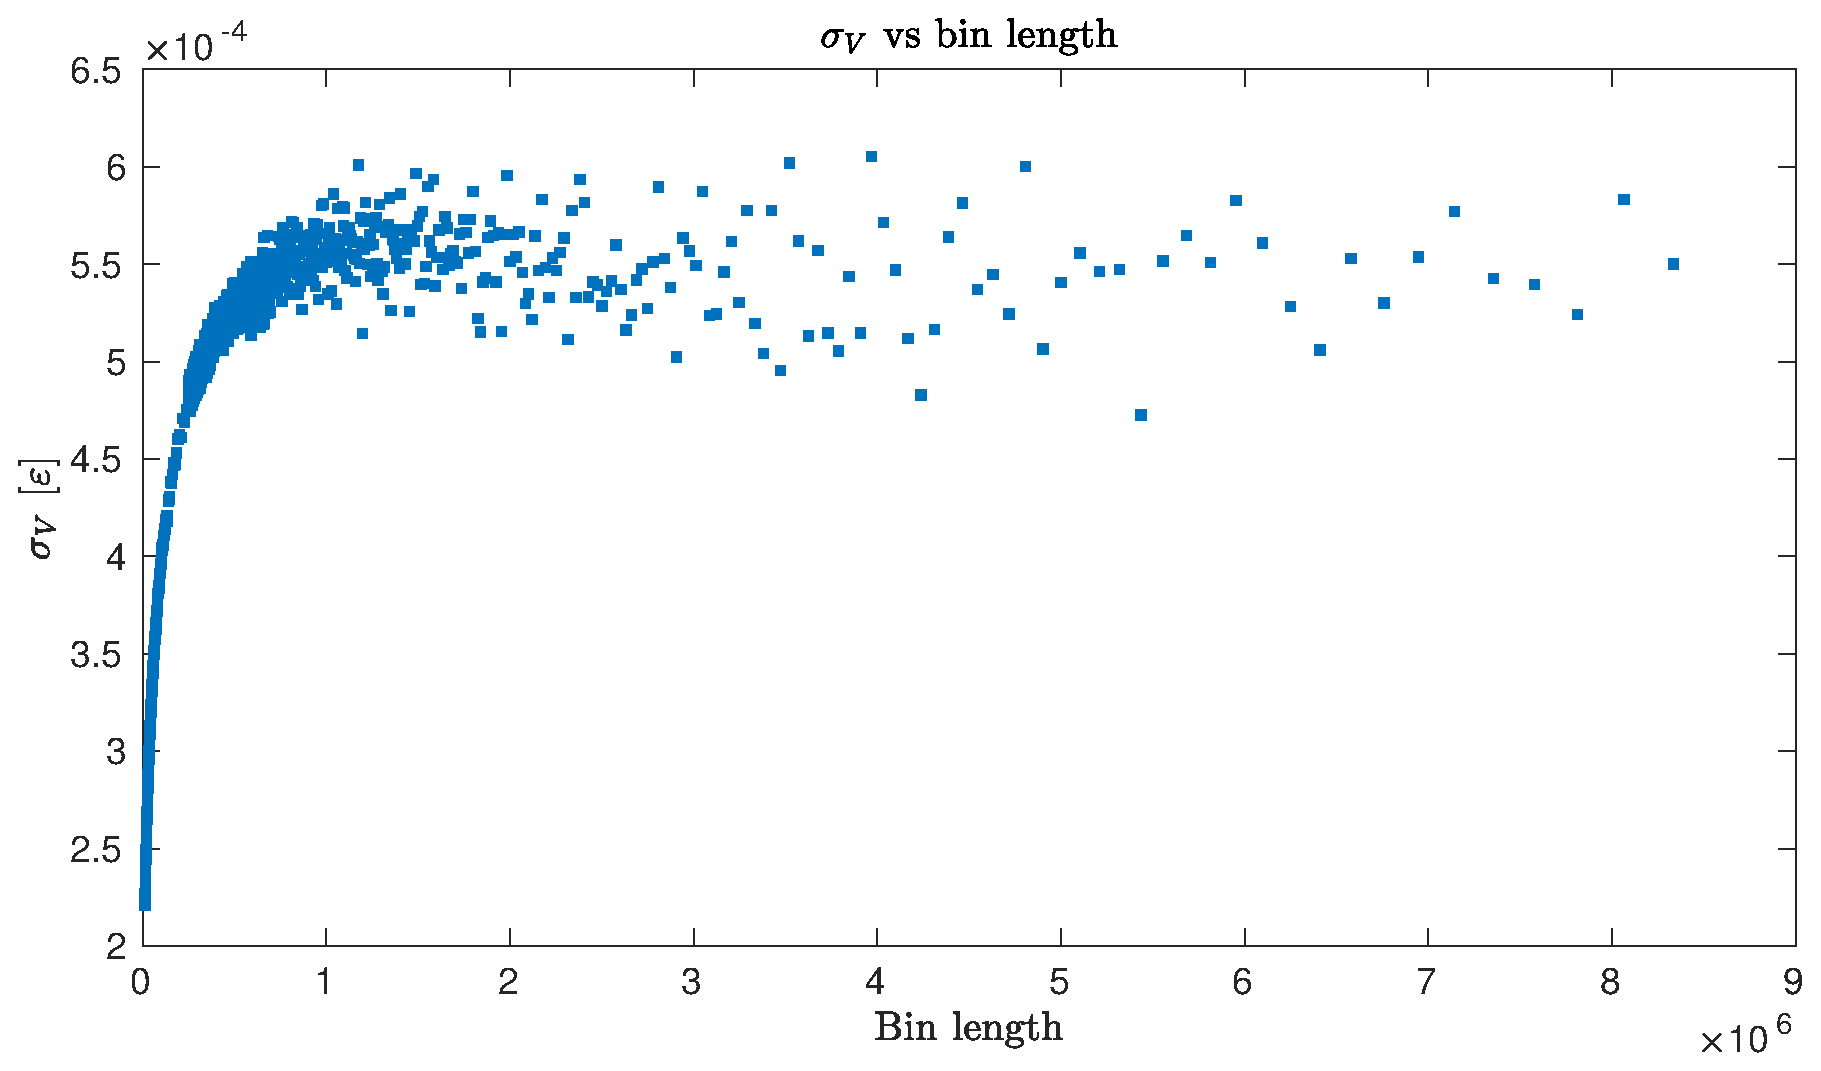
\includegraphics[width=0.9\textwidth]{binning500_example}
			\caption{Binning technique used on the data generated for the comparison with the NIST for 500 atoms, as discussed later.}
			\label{fig:binning_example}
		\end{figure}
	\end{itemize}
\end{frame}

\section{Validation against existing programs}

\begin{frame}[allowframebreaks]{Results}
	
	\begin{itemize}
		\item \textbf{Open Source Physics's LJMC}\footnote{\url{http://stp.clarku.edu/simulations/lj/mc/index.html}}
		\begin{itemize}
			\item The program simulates a 2D LJ fluid. The chosen parameters were $N=64$, $\rho = 0.5$, $T = 5.0$.
			\item The program is written in Java, therefore it's pretty slow even for a 2D simulation. 3D simulations are not supported.
			\item Results:
			\begin{table}
				\begin{tabular}{lccc}
					\toprule
					 & $\Braket{V}/N$ & $C_v/N$ & $\Braket{P}$ \\
					\midrule
					Me & $-0.70 \pm 0.01$ & $0.128 \pm 0.003$ & $4.024 \pm 0.004$ \\
					OSP & $-0.705 \, \pm \, ???$ & $0.137 \, \pm \, ???$ & $5.075 \, \pm \, ???$ \\
					\bottomrule
				\end{tabular}
			\end{table}
			\item OSP's program gives \alert{no uncertainty}, therefore a correct comparison is impossible.
			\item It's not clear which \alert{cutoff} are they using. It seems though that it's $L/2$.
			\item It's \emph{not clear} whether OSP's program is using or not \alert{tail corrections}.
			\item Nevertheless the potential is compatible within one standard deviation (of mine, of course); the specific heat is almost the same, although non compatible, while the pressure is completely out.
		\end{itemize}
		
		\item \textbf{Geissler\&Smit's simulator}\footnote{\url{http://www.cchem.berkeley.edu/chem195/_l_j___n_v_t_8m.html}}
		\begin{itemize}
			\item This program belongs to a suite written for the course of ``\textit{Understanding Molecular Simulations}'' held in UC Berkeley by Phillip Geissler and Berend Smit.
			\item The program is written in \MATLAB, so it cannot handle a large number of particles or a long computation. The number of steps the program could do in a reasonable time was $10^6$\footnote{In this program, each MC step involves the successive movement of all the particles.}.
			\item The chosen parameters were $N=100$, $\rho = 0.5$, $T = 2.0$.
			\item The program \emph{does not} use tail corrections.
			\item Results:
			\begin{table}
				\begin{tabular}{lccc}
					\toprule
					 & $\Braket{V}/N$ & $C_v/N$ & $\Braket{P}$ \\
					\midrule
					Me & $-3.136 \pm 0.004$ & $0.296 \pm 0.007$ & $1.05 \pm 0.01$ \\
					Me \scriptsize{(w/o TC's)} & $-2.969 \pm 0.004$ & $0.296 \pm 0.007$ & $1.22 \pm 0.01$ \\
					G\&S \scriptsize{(w/o TC's)} & $-3.153 \, \pm \, ???$ & -- & -- \\
					\bottomrule
				\end{tabular}
			\end{table}
			\item The program \emph{does not provide} any indication of the \alert{errors}.
			\item Specific heat and pressure are not computed, therefore a comparison is impossible.
			\item The results are not compatible anyway. This could be due to a low number of Monte Carlo steps in G\&S, or more likely to the absence of any thermalization steps. In the beginning the energy of the configuration is in fact much lower, and if there is not any thermalization this low energy samples are taken into account in the final mean, thus lowering its value with respect to its true equilibrium value.
		\end{itemize}
		\item \textbf{Cameron F. Abrams's simulator}\footnote{\url{http://www.pages.drexel.edu/~cfa22/msim/node19.html}}
		\begin{itemize}
			\item This program was written for the course in ``\emph{Molecular Simulations}'' held in Drexel University, Philadelphia, by Cameron Abrams.
			\item The program is written in C, which is in principle quite fast, but it \alert{lacks any optimization} due to the one-particle moves; it recalculates the whole energy every time. Therefore, it's still pretty slow.
			\item You can choose whichever value you want for the cutoff radius, but the implementation for $r_c > L/2$ is completely \alert{wrong}.
			\item The program uses tail corrections from \cite{Frenkel2002}.
			\item The chosen parameters were $N=100$, $\rho = 0.5$, $T = 2.0$ and $r_c = L/2$.
			\item Results:
			\begin{table}
				\begin{tabular}{lccc}
					\toprule
					 & $\Braket{V}/N$ & $C_v/N$ & $\Braket{P}$ \\
					\midrule
					Me & $-3.136 \pm 0.004$ & $0.296 \pm 0.007$ & $1.05 \pm 0.01$ \\
					Abram & $-3.137 \, \pm \, ???$ & -- & $1.05 \, \pm \, ???$ \\
					\bottomrule
				\end{tabular}
			\end{table}
			\item The results match within one standard deviation, but again Abram's program gives \alert{no uncertainty}.
		\end{itemize}
		\item \textbf{Johnson et al.'s simulation data}\footnote{\cite{Johnson1993}.}
		\begin{itemize}
			\item The chosen parameters were $N=500$, $\rho = 0.5$, $T = 2.0$ and $r_c = 5$.
			\item The simulation includes tail corrections.
			\item The equilibration is done with $\SI{2.5e6}{}$ steps and the production is done with $\SI{1.5e7}{}$ steps. The displacement is adjusted such that the acceptance is about $\SI{40}{\percent}$.
			\item Notice that, if one chooses a cutoff $r_c=L/2$, $N=500$ and $\rho=0.5$ corresponds to $r_c=5$. So, my program can perfectly reproduce the chosen parameters without any modification.
			\item Results:
			\begin{table}
				\begin{tabular}{lccc}
					\toprule
					 & $\Braket{V}/N$ & $C_v/N$ & $\Braket{P}$ \\
					\midrule
					Me & $-3.149 \pm 0.001$ & $0.316 \pm 0.003$ & $1.071 \pm 0.003$ \\
					Johnson et al. & $-3.149 \pm 0.002$ & -- & $1.069 \pm 0.003$ \\
					\bottomrule
				\end{tabular}
			\end{table}
		\end{itemize}
		\item \textbf{NIST simulation data}\footnote{\url{https://mmlapps.nist.gov/srs/LJ_PURE/mc.htm}}
		\begin{itemize}
			\item The data provided by NIST (The US National Institute of Standards and Technology) is intended to be a guide for \alert{testing codes}. The organization provides simulation results of the LJ fluid obtained with many different techniques.
			\item The chosen parameters were $N=500$, $\rho = 0.9$, $T = 0.9$ and $r_c = 3$.
			\item The simulation includes tail corrections.
			\item The equilibration is done with $\SI{5e7}{}$ steps and the production is done with $\SI{2.5e8}{}$ steps. The uncertainties are obtained from block averages of $\SI{5e7}{}$ trials and the displacement is adjusted such that the acceptance is about $\SI{40}{\percent}$.
			\item Notice that, if one chooses a cutoff $r_c=L/2$, $N=500$ and $\rho=0.9$ corresponds to $r_c \simeq 4.11$. So, if one wants to have $r_c=3$ and pretends to ignore size effects, $N=194$ should be enough. We will see if ignoring size effects will lead to an incompatible result or not.
			\item If we reduce the number of atoms, we also have to reduce the number of steps in order to have comparable simulations; $\SI{2.5e8}{}$ steps for $N=194$ will correspond to a higher number of moves per atom than for $N=500$. To have the same number of moves per particle, we have to use roughly $\SI{2e7}{}$ equilibration steps and $\SI{1e8}{}$ production steps.
			\item Results:
			\begin{table}
				\begin{tabular}{lccc}
					\toprule
					 & $\Braket{V}/N$ & $C_v/N$ & $\Braket{P}$ \\
					\midrule
					Me \scriptsize{(N=194)} & $-6.179 \pm 0.001$ & $1.219 \pm 0.003$ & $2.56 \pm 0.01$ \\
					Me \scriptsize{(N=500)} & $-6.1773 \pm 0.0006$ & $1.218 \pm 0.002$ & $2.582 \pm 0.003$ \\
					NIST \scriptsize{(N=500)} & $-6.1773 \pm 0.0016$ & -- & $2.58 \pm 0.01$ \\
					\bottomrule
				\end{tabular}
			\end{table}
		\end{itemize}
	\end{itemize}
	
\end{frame}

\begin{frame}{Summary of the comparison}
	\begin{itemize}
		\item {\color{myred} \makebox[9cm][l]{\sout{Open Source Physics's LJMC}} \Large\Frowny}\\
		{\footnotesize{\alert{Reason:} no uncertainties}}
		\item {\color{myred} \makebox[9cm][l]{\sout{Geissler\&Smit's simulator}} \Large\Frowny}\\
		{\footnotesize{\alert{Reason:} no uncertainties, incompatible measurements}}
		\item {\color{myred} \makebox[9cm][l]{\sout{Cameron F. Abrams's simulator}} \Large\Frowny}\\
		{\footnotesize{\alert{Reason:} no uncertainties}}
		\item {\color{mygreen} \makebox[9cm][l]{Johnson et al.'s simulation data} \Large\Smiley}\\
		{\footnotesize{Within 1 std}}
		\item {\color{mygreen} \makebox[9cm][l]{NIST simulation data} \Large\Smiley}\\
		{\footnotesize{Within 1 std}}
	\end{itemize}
\end{frame}


\section{Running the simulation}

\begin{frame}[allowframebreaks]{First checks}
	
	Now, let's say just a few words about the simulation and how we can check that we are doing a good run.
	
	\begin{itemize}
		\item The \alert{first thing} to choose, for a given system configuration, is the maximum \alert{step length}.
		\item Monte Carlo simulations, at this level, are much like a ``cuisine experiment'': you try some values until you get some nice results.
		\item A typical \emph{rule of thumb} for the choice of the step length is that the percentage of accepted steps is \alert{around $\SI{50}{\percent}$}, or even $\SI{40}{\percent}$. This is because
		\begin{itemize}
			\item If the step is too small (acceptance around $\SI{100}{\percent}$), then we are not sure that we are sampling all the sampling region (included points near the borders), and odds are that we are just wandering around a very small region of the sampling region, were all our moves are accepted.
			\item If the step is too large (acceptance around $\SI{0}{\percent}$ then we are jumping like \emph{crazy giant kangaroos}, mostly hitting points outside the sampling region.
		\end{itemize}
		\item The \alert{second thing} to choose is number of Monte Carlo steps and the number of \alert{thermalization steps}.
		\item There are various things we can look at to choose the proper values, but the one that I always use is to check the \alert{distribution of the samples}. You can do that \emph{very easily} even while the program is running, by just doing an \alert{histogram} of the samples with a sufficient number of bins (in these simulations, I was usually taking 1000 bins).
		\item What you should obtain is a \emph{good-looking} Gaussian-like distribution.
		\begin{itemize}
			\item If you don't obtain such a distribution but you instead obtain a flat distribution or something worse, that your Monte Carlo algorithm is \emph{wrong.}
			\item If you obtain something like two or more near Gaussians, then it means that you are \alert{not doing enough thermalization} steps. What happens is that the system has found a \emph{local minimum}, which is sampled for a certain amount of time. Then, the system finds a way out to a newer minimum (which can be again local or global) and samples it in the remaining Monte Carlo steps. To avoid this, you should increase the number of thermalization steps. Beware that you should always do a check like this, since the thermalization is not always obvious!
			\item The remaining thing, which is the number of Monte Carlo steps (after the thermalization), controls the \alert{smoothness} of the distribution. If you do few samples, then the borders of your distribution will be very \emph{saw-like}; a good number of samples, instead, is such that the borders of the distribution appear almost like continuous, smooth lines.
		\end{itemize}
	\end{itemize}
	
\end{frame}

\begin{frame}{A bad-looking Gaussian}
	\begin{figure}
		\centering
		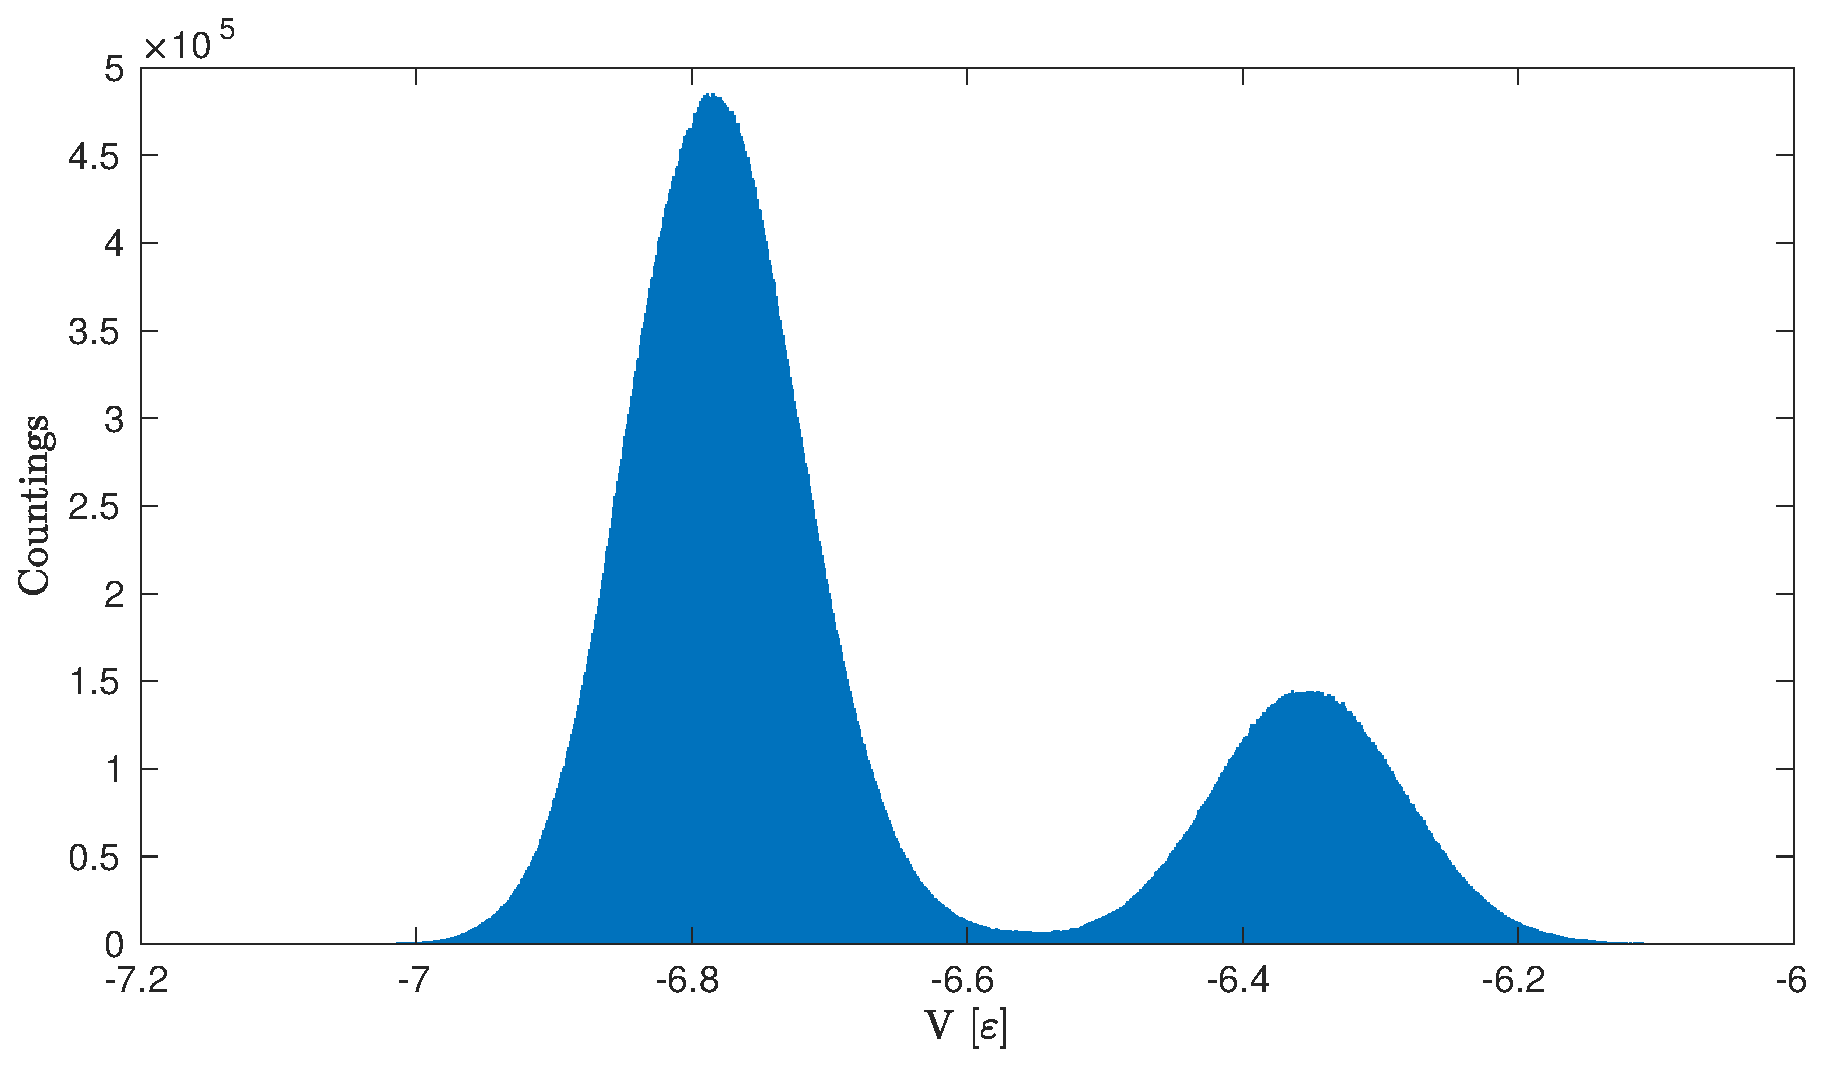
\includegraphics[width=\textwidth]{distribution_bad}
		\caption{Example in which the thermalization steps are not enough.}
		\label{fig:example_distribution_bad}
	\end{figure}
\end{frame}

\begin{frame}{A good-looking Gaussian}
	\begin{figure}
		\centering
		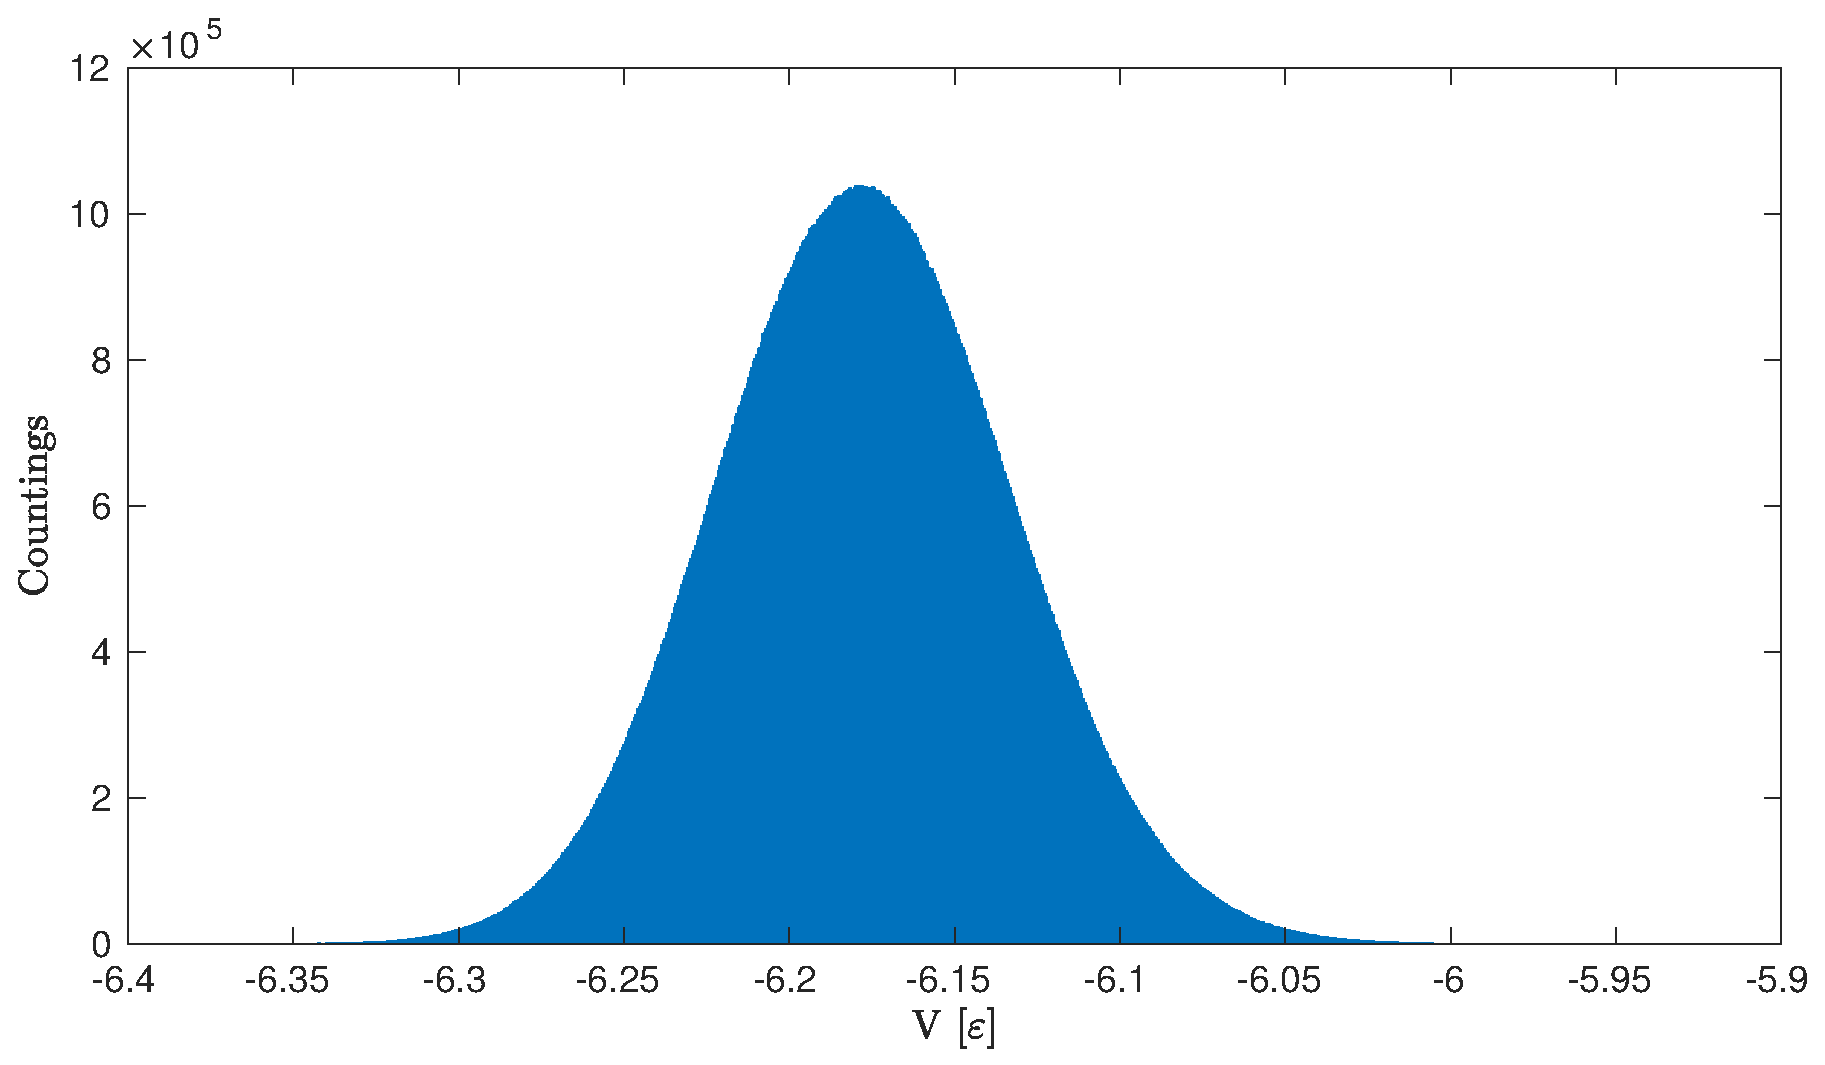
\includegraphics[width=\textwidth]{distribution500}
		\caption{Samples distribution for $N=500$, same configuration used for NIST comparison.}
		\label{fig:example_distribution_good}
	\end{figure}
\end{frame}

\begin{frame}{Other important checks}

	There are two more things worth checking:
	\begin{itemize}
		\item the \alert{mean value} of the samples over the MC time;
		\item the \alert{autocorrelation} of the samples.
	\end{itemize}
	
	The first one is a reflection of the distribution of the samples; it's an easier way to check if the mean value of the observable we are sampling is stabilized to an almost constant value. If it is not, it means that either we have too few thermalization steps or we don't have a sufficient number of Monte Carlo steps. In general, this is a signal that we have to increase the steps; however, in my opinion it's easier to distinguish between thermalization steps and production steps by looking at the distribution.
	
	The autocorrelation is \emph{very important} because it tells us if the set of samples is large enough such that the samples themselves can be considered not correlated to each other. 

\end{frame}

\begin{frame}{Mean value over time}
	\begin{figure}
		\centering
		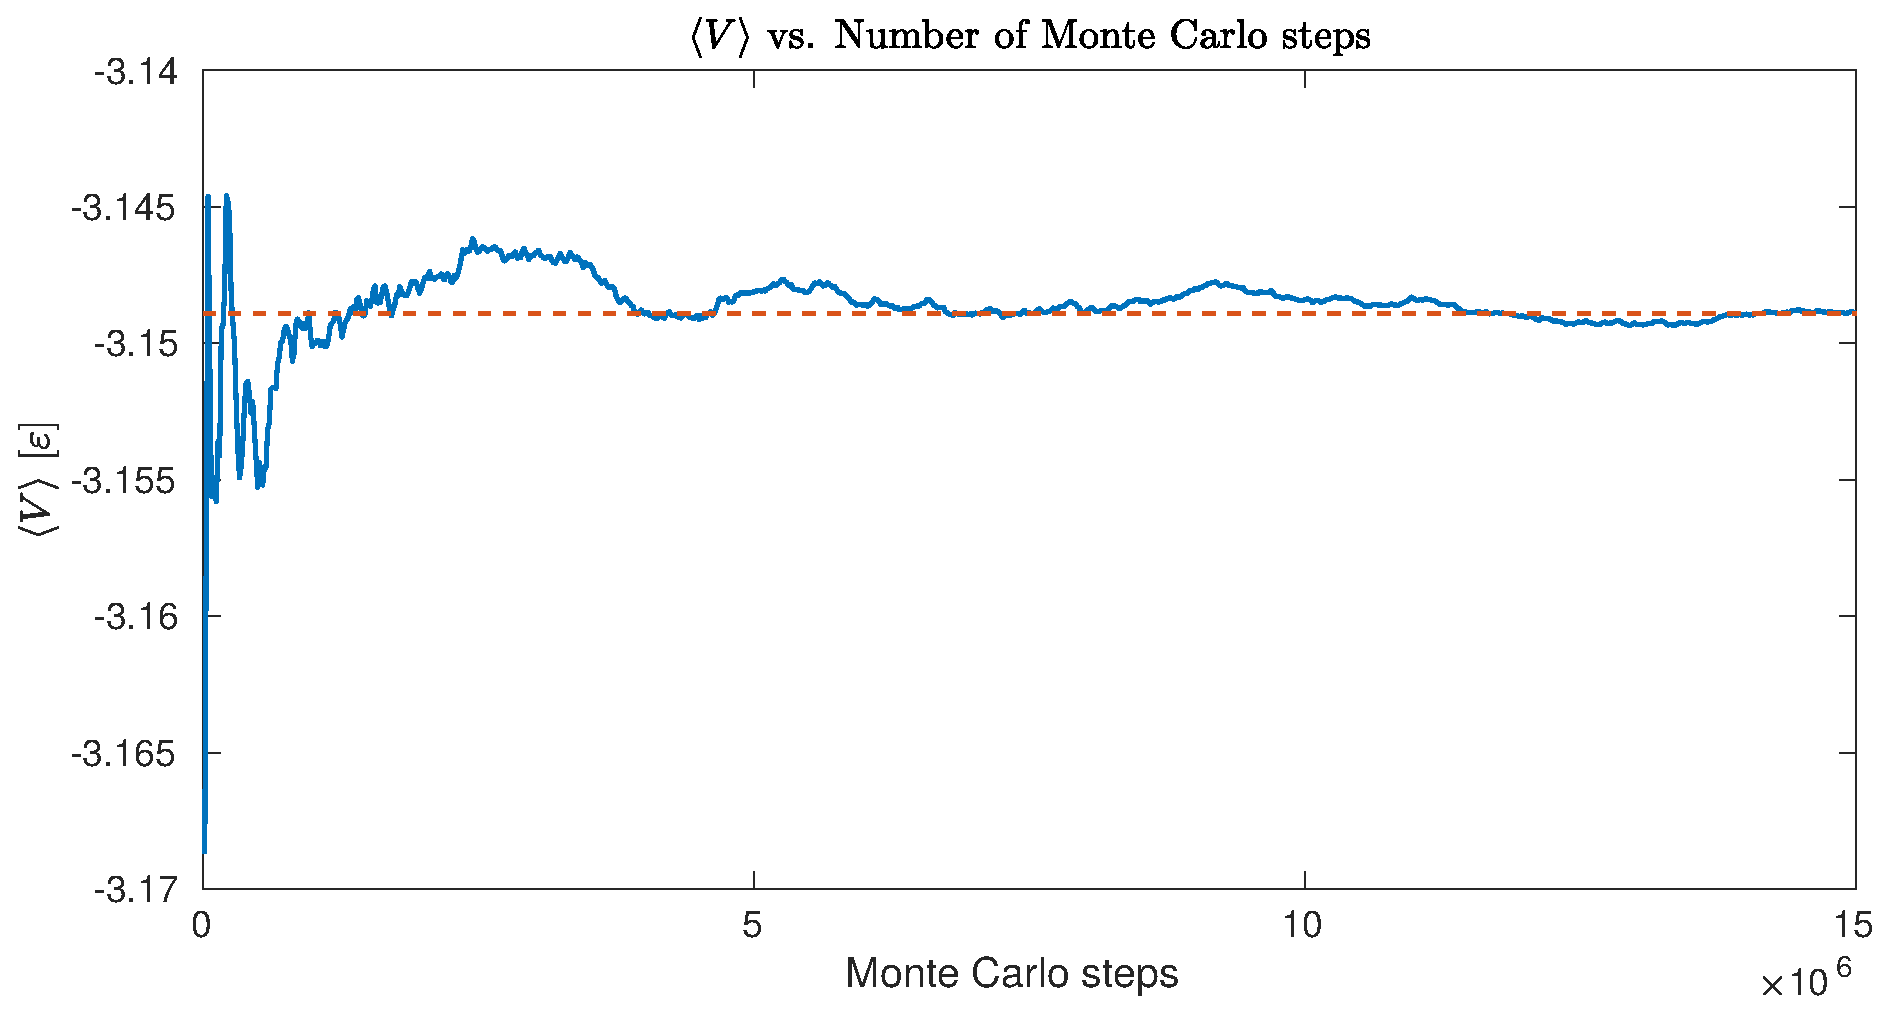
\includegraphics[width=\textwidth]{meanvalue_example}
		\caption{Mean value of the potential over the Monte Carlo time. The configuration is the same used for the comparison with \cite{Johnson1993}.}
		\label{fig:meanvalue_example}
	\end{figure}
\end{frame}

\begin{frame}{Autocorrelation}
	\begin{figure}
		\centering
		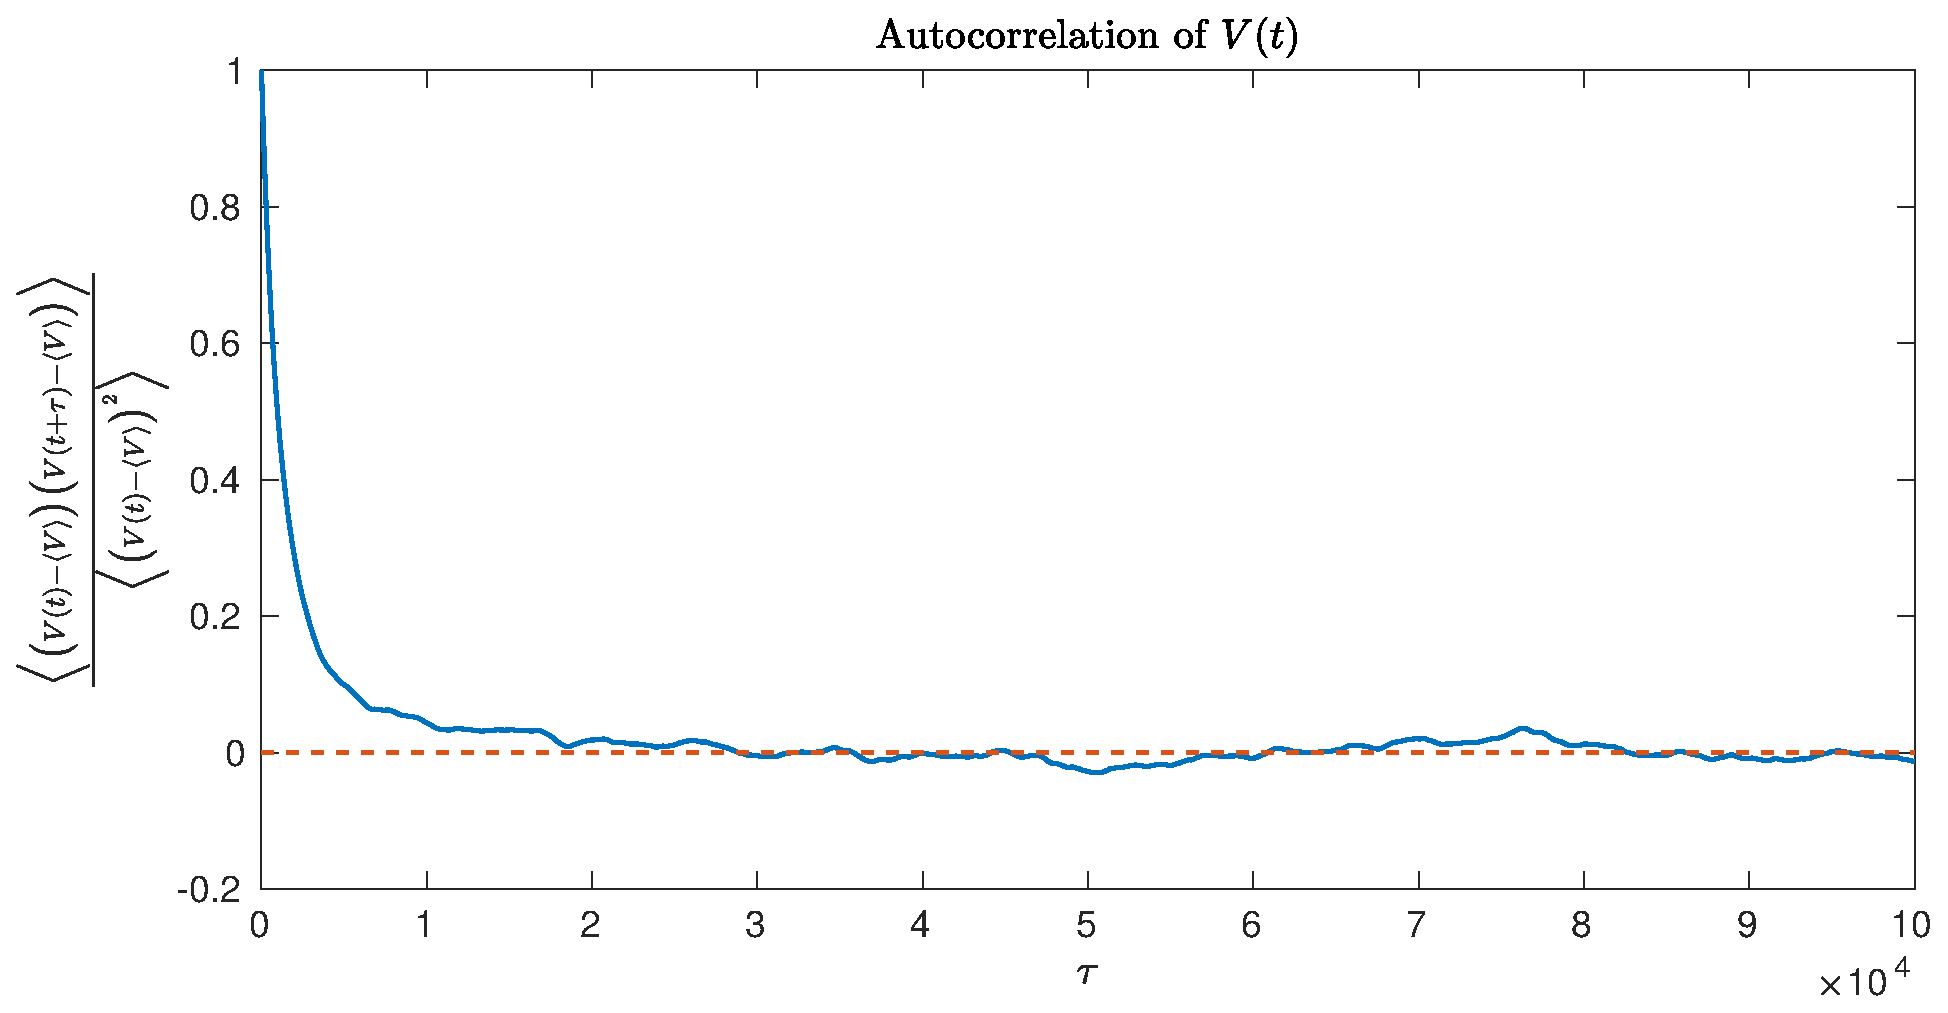
\includegraphics[width=\textwidth]{autocorrelation_example}
		\caption{Autocorrelation of the sample. The configuration is the same used for the comparison with \cite{Johnson1993}.}
		\label{fig:autocorrelation_example}
	\end{figure}
\end{frame}


\section{Isochores}

\begin{frame}{$\Braket{V}$ vs $T$}
	\begin{figure}
		\centering
		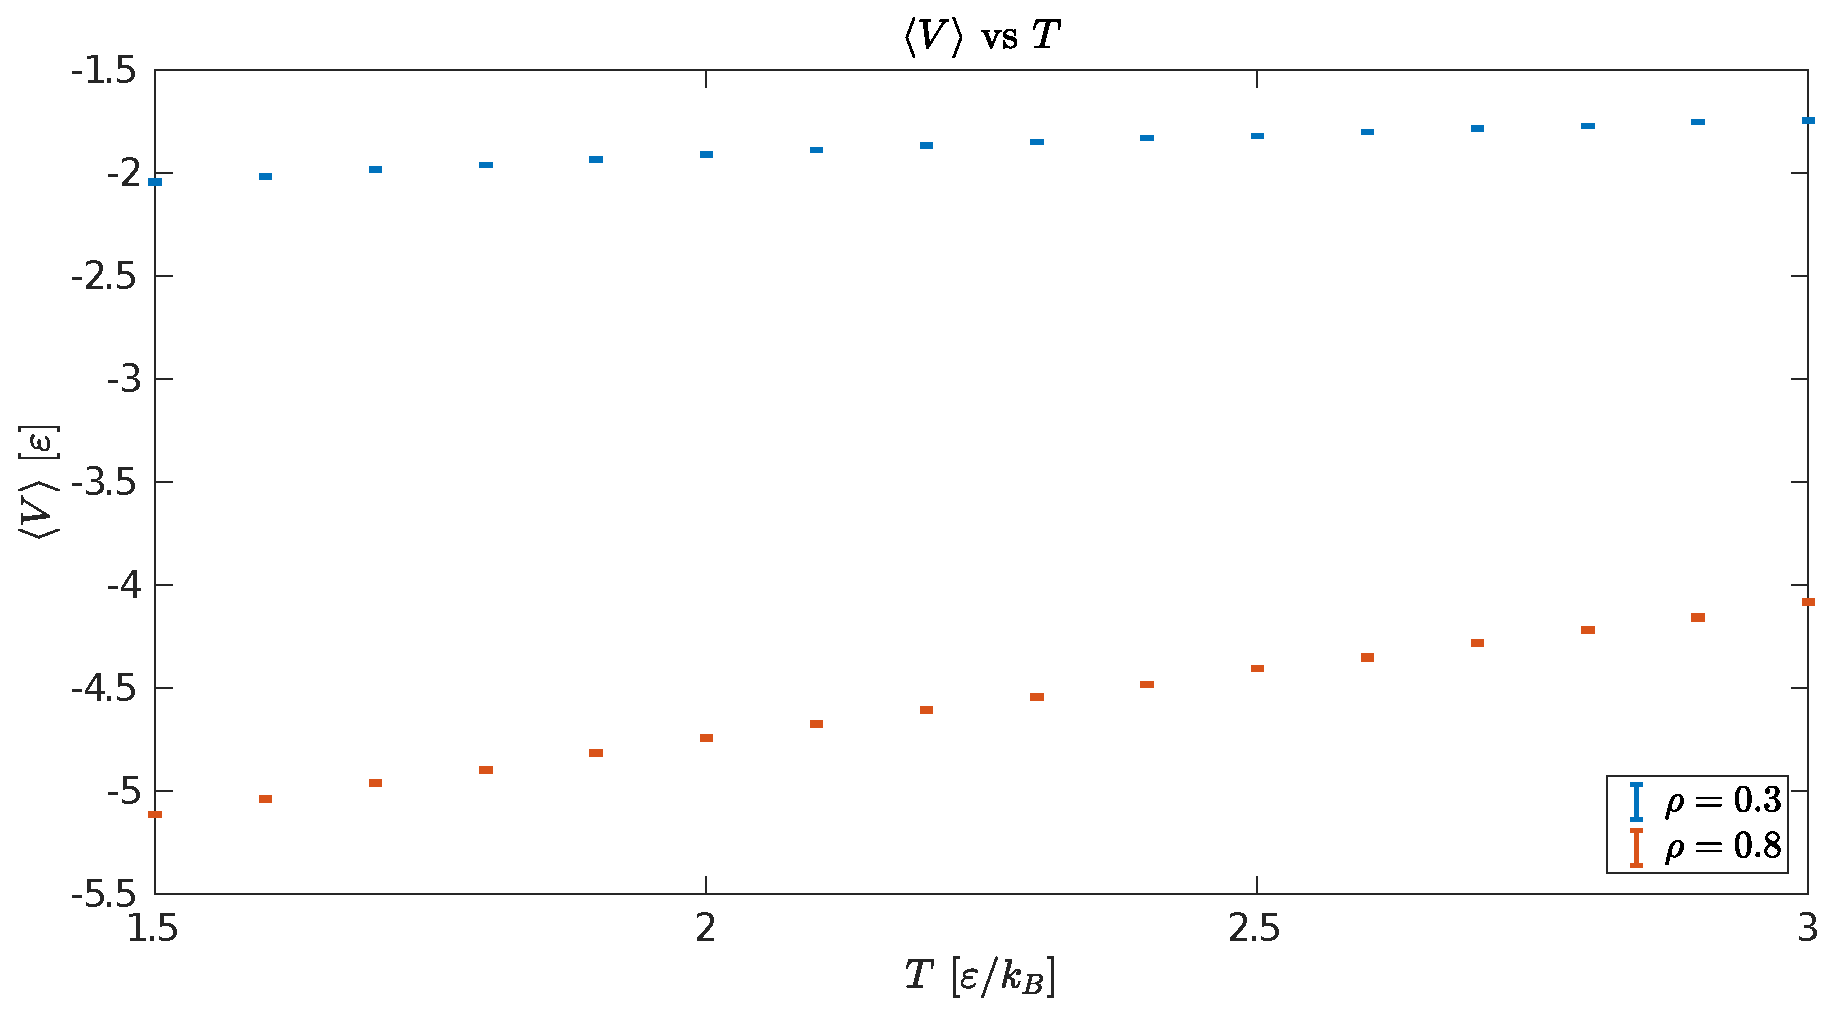
\includegraphics[width=\textwidth]{V_vs_T}
		\caption{Mean value of the potential as a function of $T$ for different values of the density.}
		\label{fig:V_vs_T}
	\end{figure}
\end{frame}

\begin{frame}{$\Braket{P}$ vs $T$}
	\begin{figure}
		\centering
		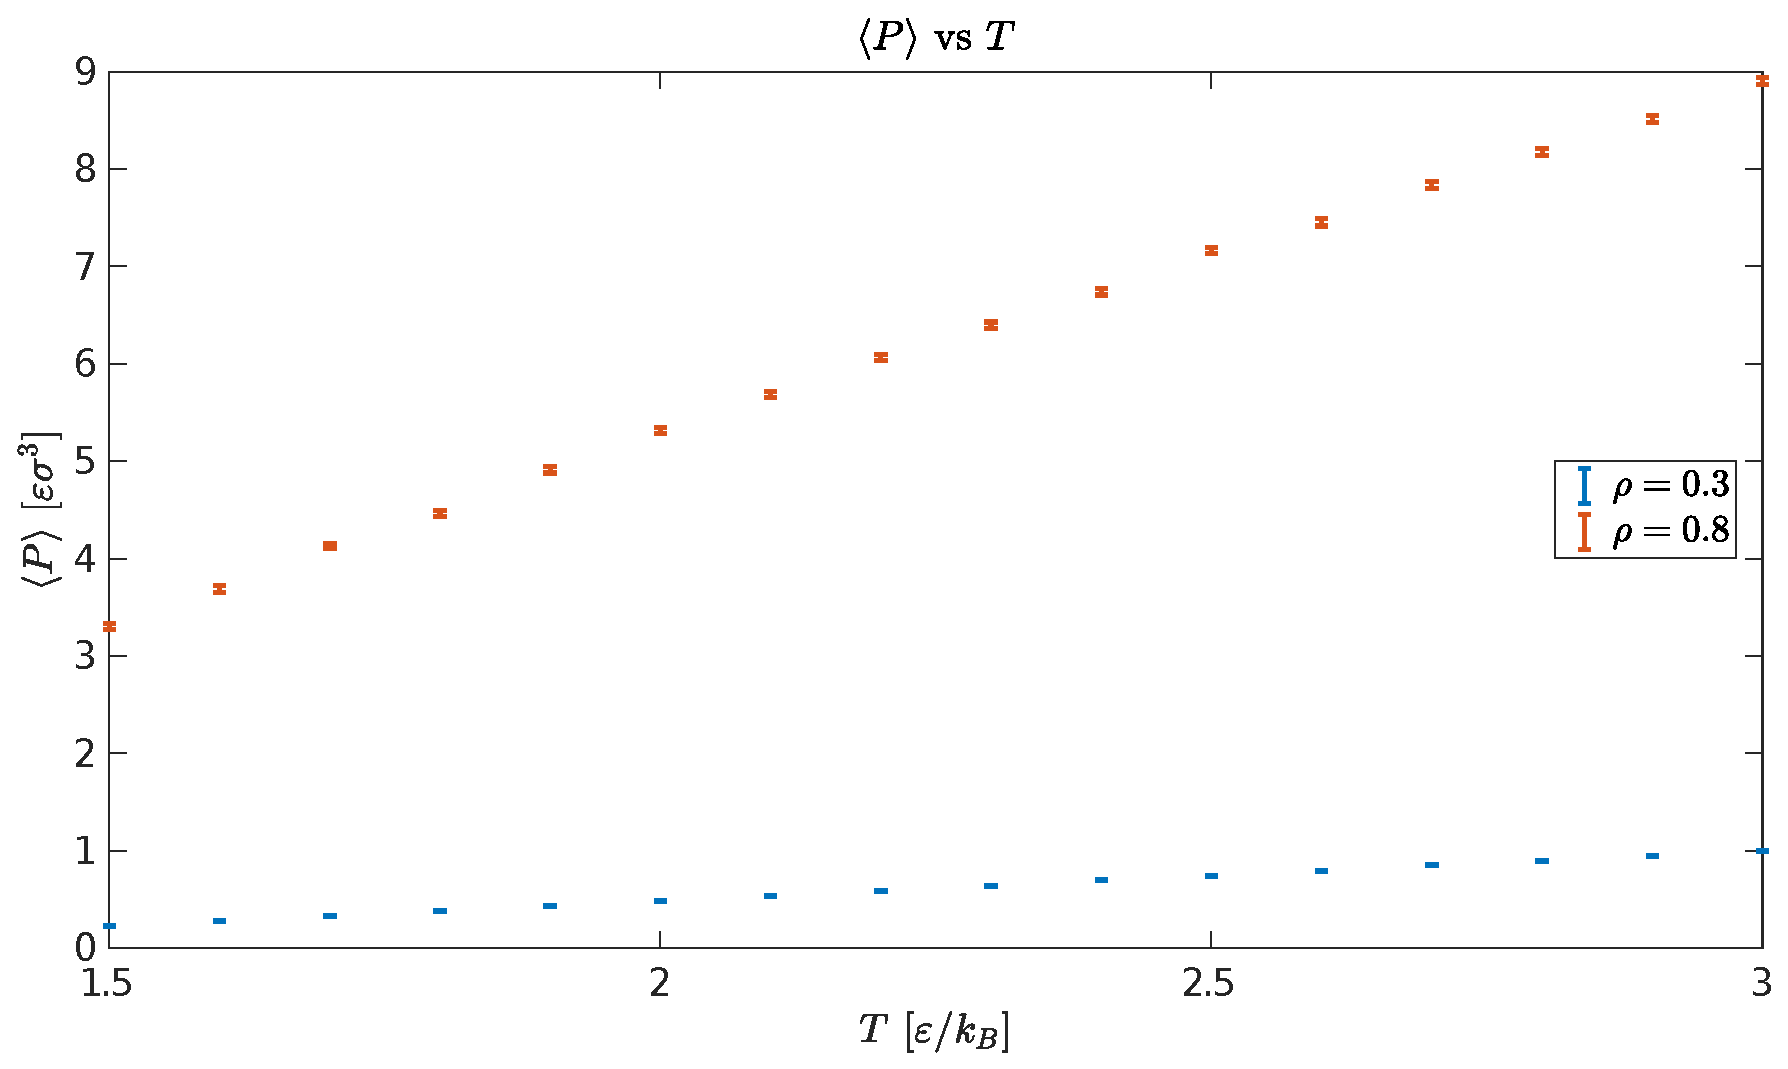
\includegraphics[width=\textwidth]{P_vs_T}
		\caption{Mean value of the pressure as a function of $T$ for different values of the density.}
		\label{fig:P_vs_T}
	\end{figure}
\end{frame}

\begin{frame}{$\Braket{C_V}$ vs $T$}
	\begin{figure}
		\centering
		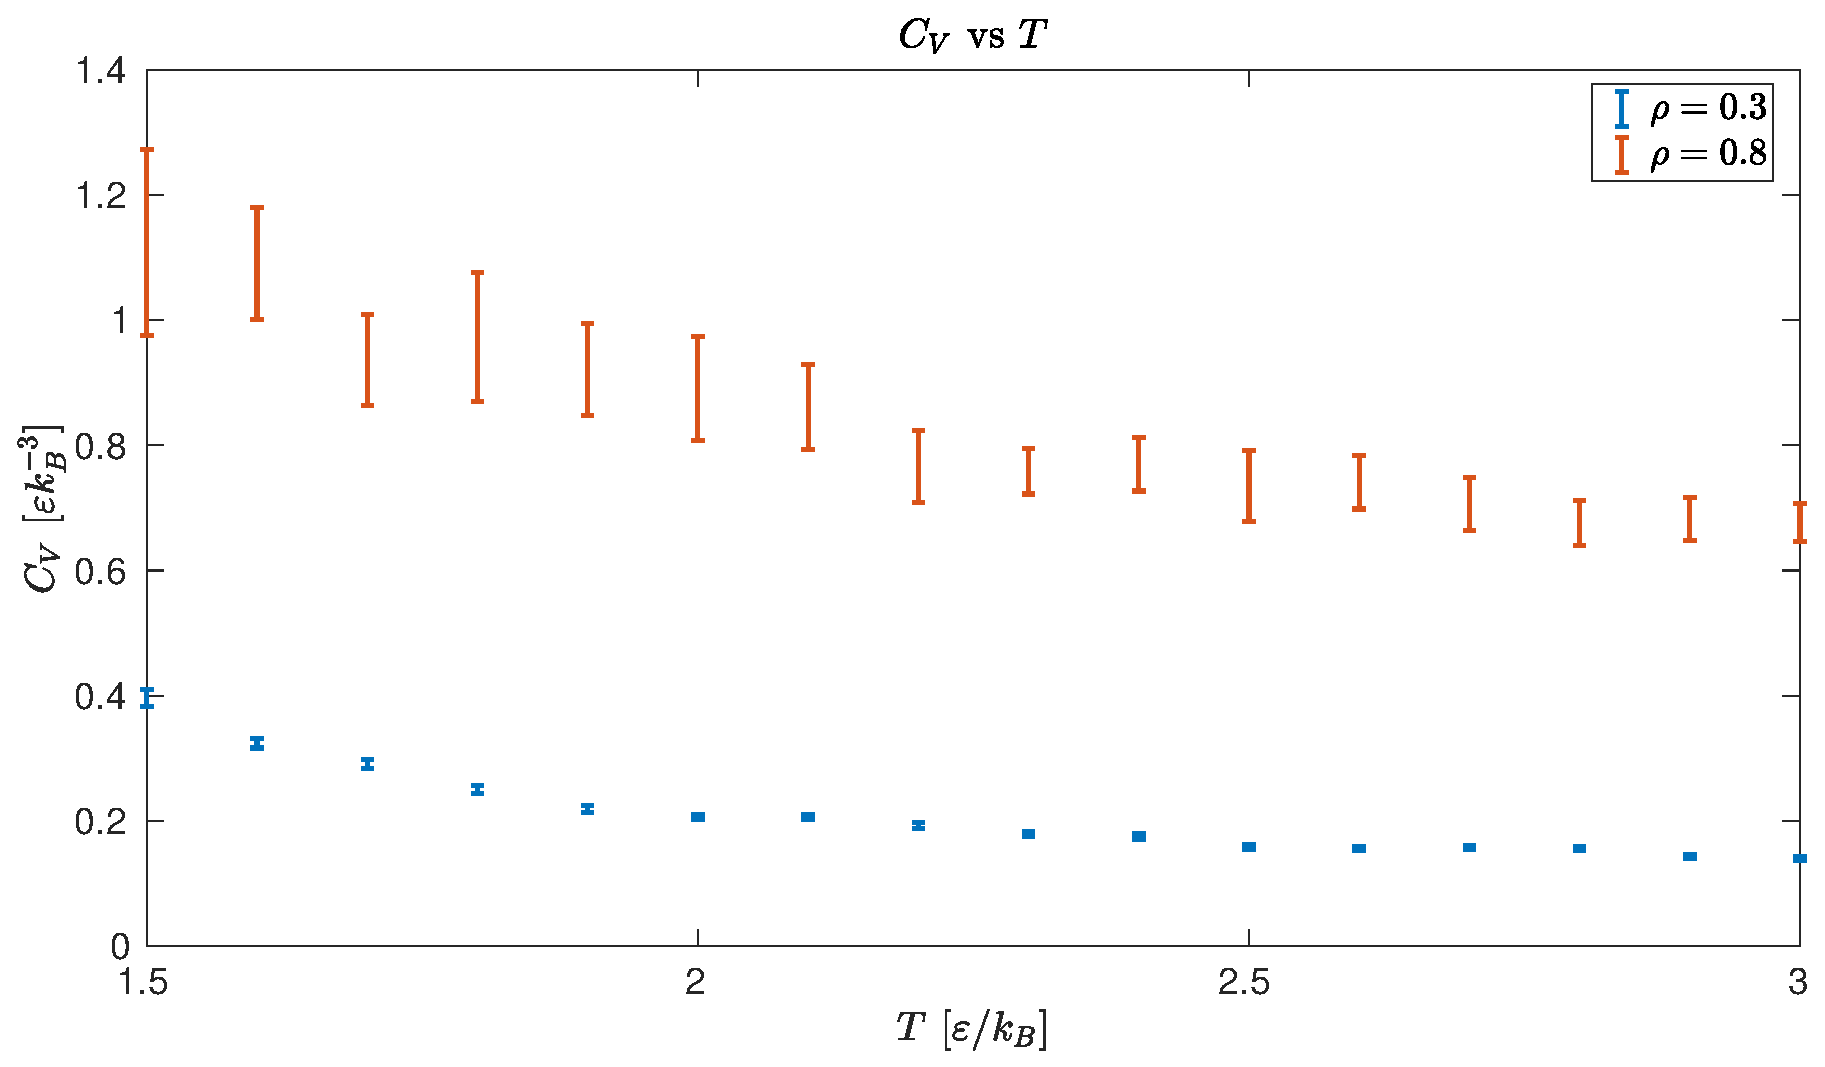
\includegraphics[width=\textwidth]{Cv_vs_T}
		\caption{Specific heat as a function of $T$ for different values of the density.}
		\label{fig:Cv_vs_T}
	\end{figure}
\end{frame}

\begin{frame}[allowframebreaks]{Remarks on the specific heat}

	Warning: in the previous figures, potential and specific heat have to be understood \emph{per particle}. I also left out the kinetic contribution to the specific heat (per particle), which is $\frac{3}{2}R$, because the kinetic energy doesn't enter into the problem.
	
	The specific heat was calculated through the fluctuations of the potential as
	\begin{equation}
		C_V = \frac{\Braket{V^2}-\Braket{V}^2}{k_BT^2}.
		\label{eq:Cv_fluctuations}
	\end{equation}
	However, we know it can also be calculated as
	\begin{equation}
		C_V = \frac{\partial \Braket{V}}{\partial T}.
	\end{equation}
	This second expression is \emph{not convenient} in our case, because it requires the knowledge of $\Braket{V}$ at two points that are infinitesimally near. In fact:
	\begin{enumerate}
		\item if the two points are too near, the result of the derivative is dominated by the uncertainty on $\Braket{V}$;
		\item if the two points are not near enough, the line connecting them will not be a good approximation of the potential curve and therefore the discrete derivative will not be a good approximation of the real one.
	\end{enumerate}
	
	What one can do to improve this situation is to calculate $\Braket{V}$ for different values of $T$ around the temperature of interest and then derive the curve \alert{fitting} these points. This improvement, however, comes at a cost: we have to run multiple simulations for different $T$'s just to know the specific heat at a \emph{single} value of the temperature! Moreover, the specific heat calculated in this way has still a considerable error due to the confidence intervals of the fitting parameters. In the end, the calculation through the fluctuations is more convenient because:
	\begin{enumerate}
		\item It requires a \alert{single calculation}.
		\item The numerator of equation \eqref{eq:Cv_fluctuations} is basically the \emph{standard deviation} of the distribution of the potential, which has a well-defined value with infinite precision in the limit of an infinite simulation. Of course, we cannot do an infinite simulation; what I want to say is simply that we can obtain a result for the specific heat with a precision that is consistent with the precision we want for the other observables of the simulation, and that this precision -- for a given configuration of the system -- is uniquely determined by the length of the simulation itself.
	\end{enumerate}
	
	Note that this cannot be obtained with the analytical derivative method, because even if we have values of the potential with infinite precision then we have to calculate an infinite number of $(T,\Braket{V})$ points around the derivation point in order to have zero-error fit.
	
	In Figure \ref{fig:Cv_comparison}, we show the value of $C_V$ calculated with both methods.
	
	Beware that in the figure there should be also the \alert{confidence intervals} of the derivative of the fit. However, despite being able to plot the confidence intervals of the $\Braket{V}$-vs-$T$ fit, I couldn't manage to calculate the confidence intervals \emph{of the fit}. In other words, you should imagine a wide \alert{stripe} instead of a single line.
	
	\begin{figure}
		\centering
		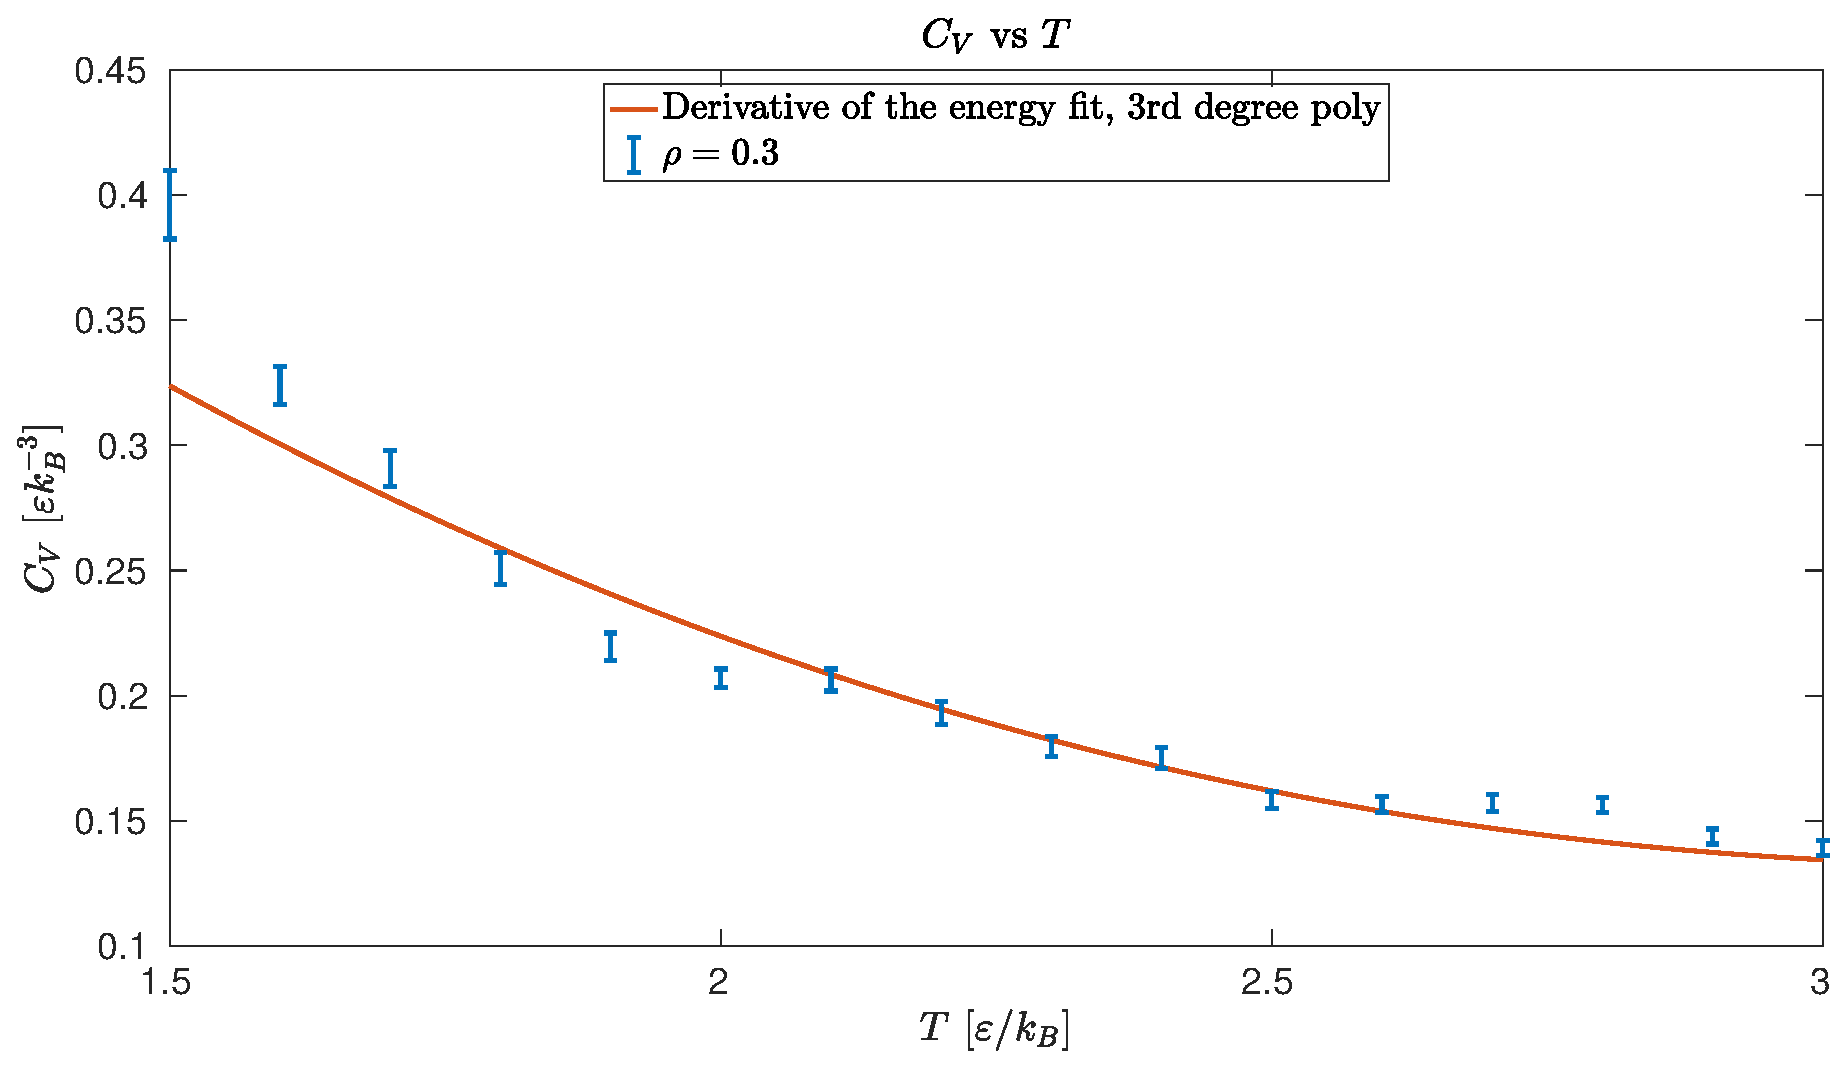
\includegraphics[width=\textwidth]{Fluctuations_vs_Analytical}
		\caption{Example of specific heat calculated with two different methods.}
		\label{fig:Cv_comparison}
	\end{figure}
	
\end{frame}


\section{Isotherms}

\begin{frame}[allowframebreaks]{Preliminaries}

	Let's now study the isotherms of the system in the pressure-density plane.
	
	In this plane, it is in fact possible to find the points that belong to the \alert{liquid-vapor coexistence curve}. Beware that this requires the knowledge of the saturation pressure, which cannot be determined by standard NVT simulations (more about this later). So, I've used tabulated data for the saturation pressure from \cite{Johnson1993} and \cite{Siderius2012} in order to compare my results to the ones found in the literature.
	
	First of all, let's put some boundaries to temperature and density that we are gonna use in the simulations.
	\begin{itemize}
		\item From the data all around the literature (e.g. \cite{Johnson1993}), I've found that for the present purposes it's enough to simulate the system for $\rho = 0.05 \div 0.9$ and $T = 0.6 \div 1.5$.
		\item I've chosen to use a cutoff $r_c \geq 3.0$, which means that for the chosen density range it's enough to use $N=200$.
		\item I've used $10^6$ thermalization steps and $10^7$ production steps.
	\end{itemize}
	
%	200 particles is enough to have rc>=3 for rho=0.05...0.9
%	In Fig1 from Smit, it seems we don't need T<0.7 or 0.6. So, let's do from 0.6 on.
%	Let's do 10^7 steps with thermalization 10^6

\end{frame}

\begin{frame}{$P$-$\rho$ isotherms}

	\begin{figure}
		\centering
		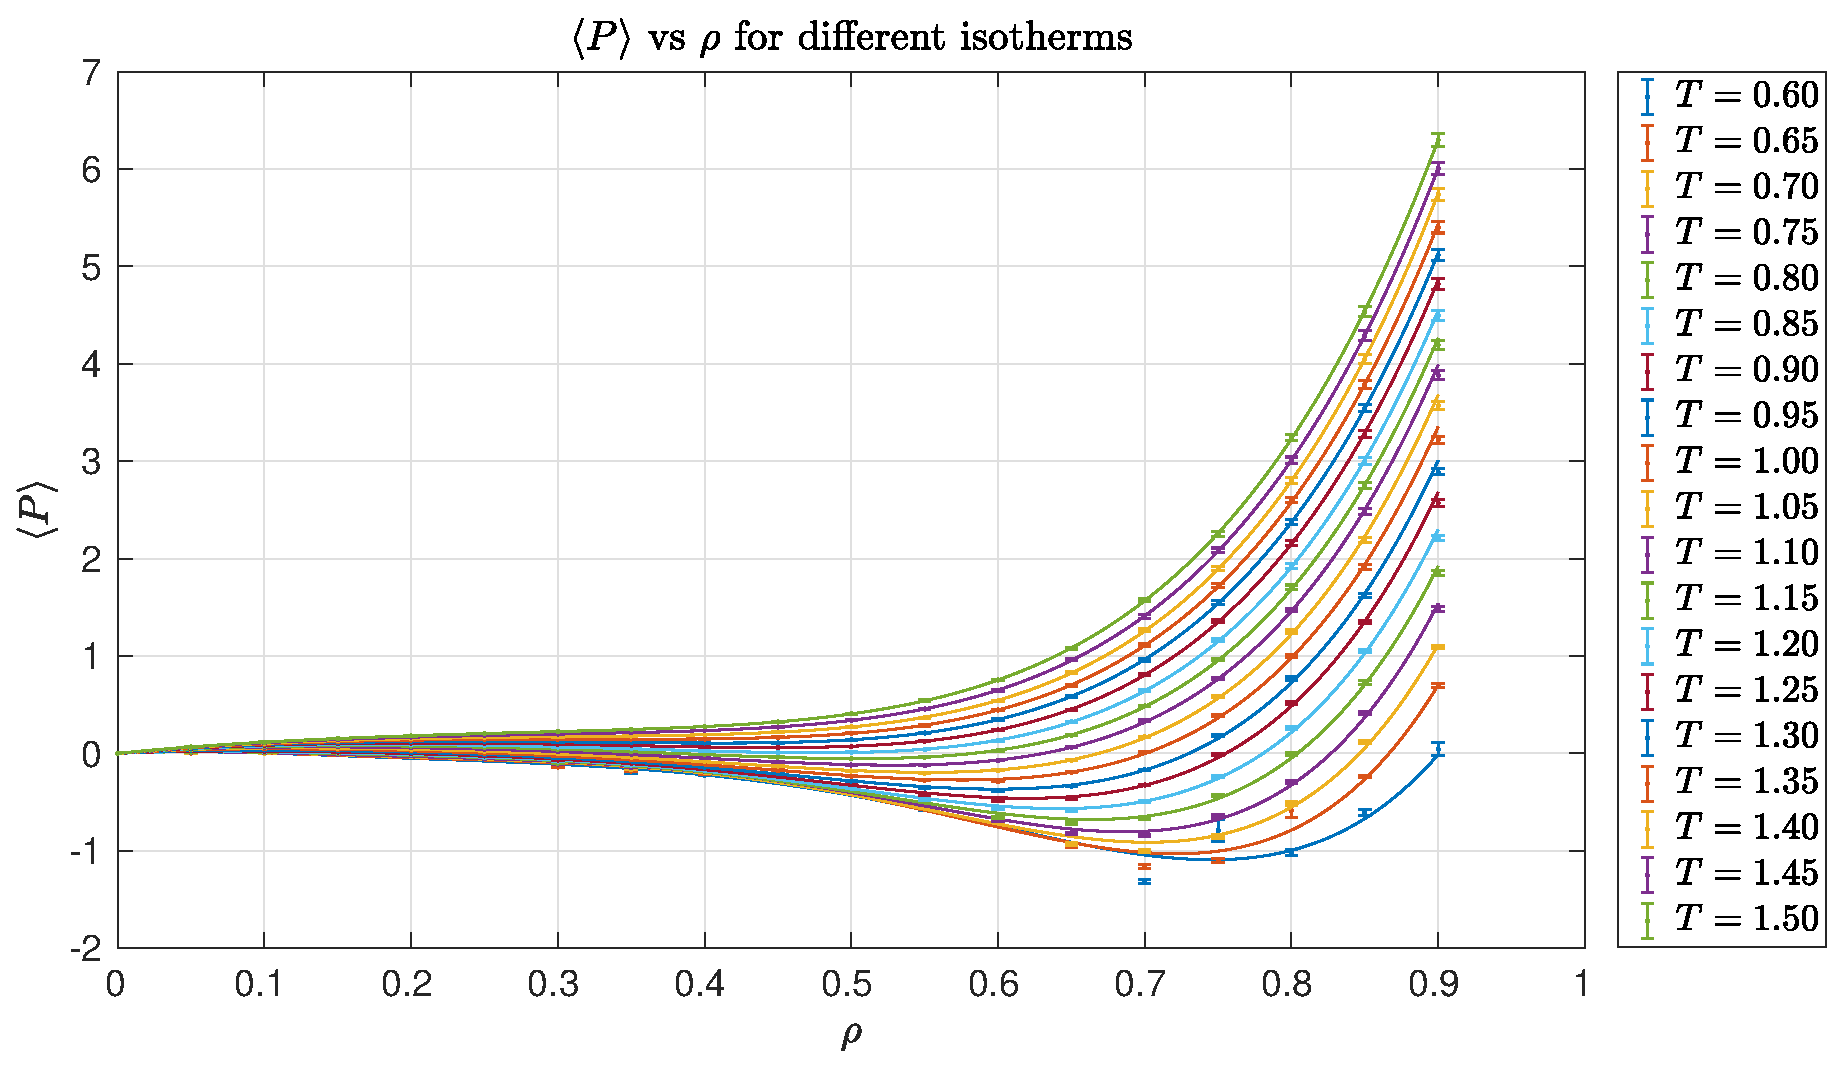
\includegraphics[width=\textwidth]{PvsRho}
		\caption{Isotherms in the $P$-$\rho$ plane.}
		\label{fig:P_vs_Rho}
	\end{figure}

\end{frame}

\begin{frame}{MBWR fit}

	\begin{figure}
		\centering
		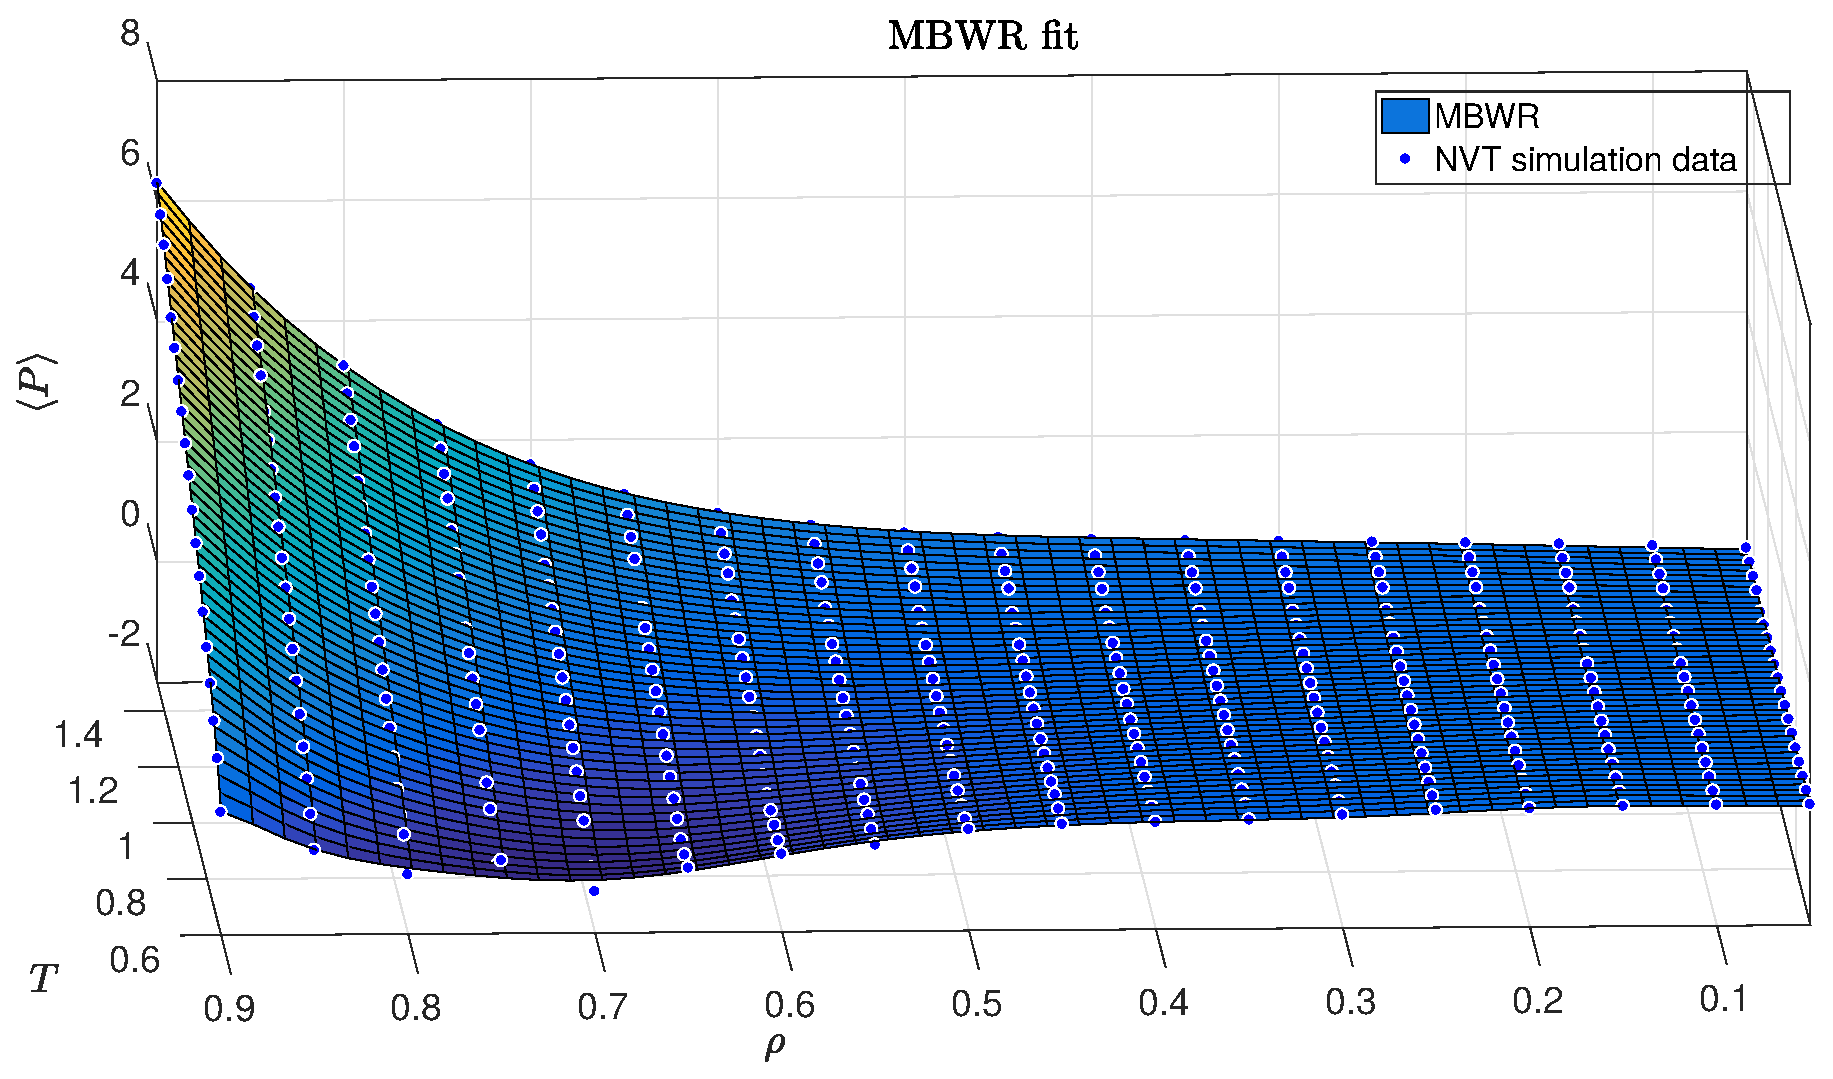
\includegraphics[width=\textwidth]{MBWR_fit}
		\caption{MBWR fit of the simulation data.}
		\label{fig:MBWR_fit}
	\end{figure}

\end{frame}

\begin{frame}{Coexistence curve}

	\begin{figure}
		\centering
		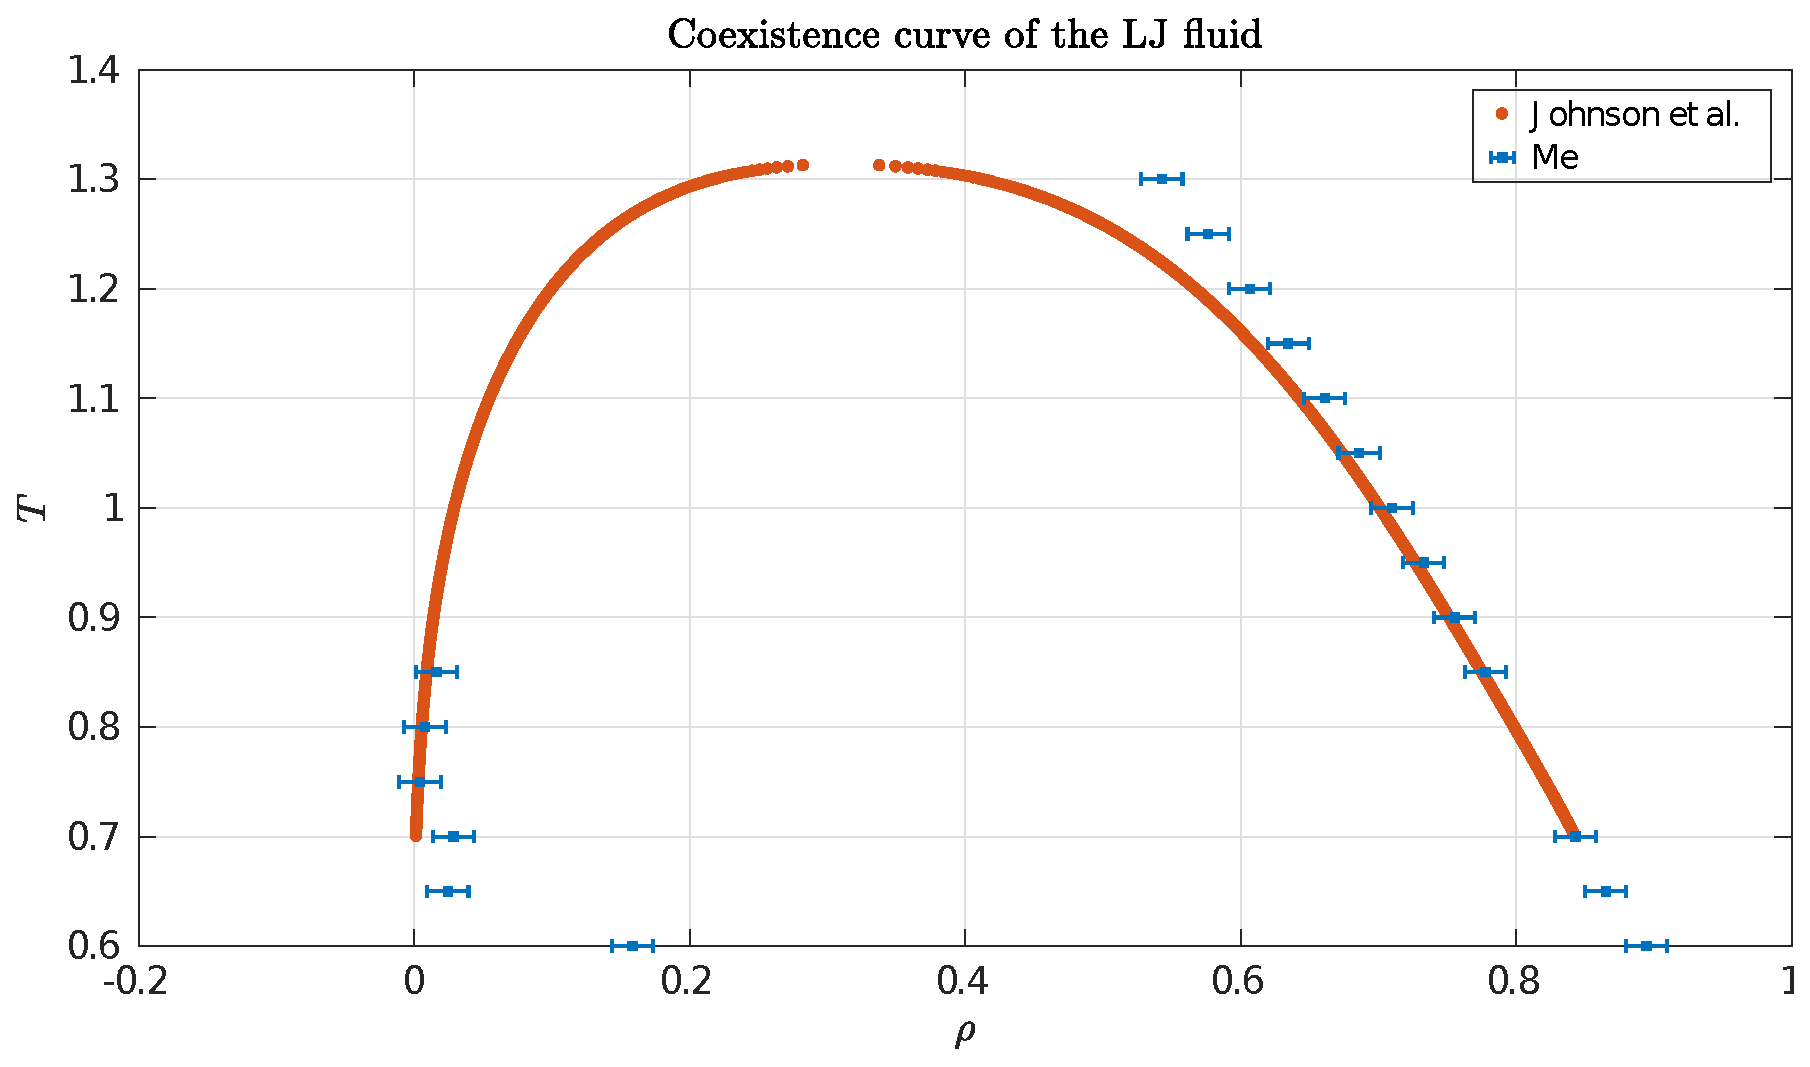
\includegraphics[width=\textwidth]{Coexistence}
		\caption{Coexistence curve of the LJ fluid.}
		\label{fig:coexistence}
	\end{figure}

\end{frame}

\begin{frame}[allowframebreaks]{Remarks}

	\begin{itemize}
		\item The MBWR (Modified Benedict-Webb-Rubin, from \cite{Nicolas1979}) fit is a 33-parameters fit with a \emph{horrible expression}. It is popular because it's relatively simple, having only one non-linear parameter out of 33.
		\item I couldn't find any low-density solution except for low temperatures. This could be due to
		\begin{itemize}
			\item poor quality of the numerical solver I've used to find the $\rho$-roots, that often cannot find multiple roots;
			\item hard to keep the acceptance around $\SI{40}{\percent}$ for the low-density/high-temperature region;
			\item shortage of points in the low-density region, where the corresponding pressure range is really small.
		\end{itemize}
		\item The agreement between the data from \cite{Johnson1993} and the results of my simulation are pretty good in the high-density region, except for the points towards the critical point. This could be due to the fact that:
		\begin{itemize}
			\item Towards the critical temperature, the $P$-$\rho$ curves gets flatter and flatter in the coexistence region. Therefore, the error obtained from using the above procedure is actually much higher than the reported one.
			\item I've used too few particles in the calculations, 200 against the 864 of \cite{Johnson1993}.
		\end{itemize}
		\item As a general thing, it is not a good idea to use these standard NVT simulations to determine the vapor-liquid coexistence curve, as explained in \cite{Frenkel2002}.
		\begin{itemize}
			\item In the coexistence region, the pressure is \emph{not constant} as instead one would expect. That's because for small systems as the one studied, the free-energy cost associated to the creation of the liquid-vapor interface is so high that the system prefers not to separate at all.
			\item For these kind of purposes, one could for example use the ``Gibbs ensemble method'', described in Chapter 8 of \cite{Frenkel2002}. Two systems are put in contact, and apart from the \emph{particle displacement}, other possible moves are also \emph{volume change} and \emph{particle exchange}.
		\end{itemize}
	\end{itemize}
	
	\begin{figure}
		\centering
		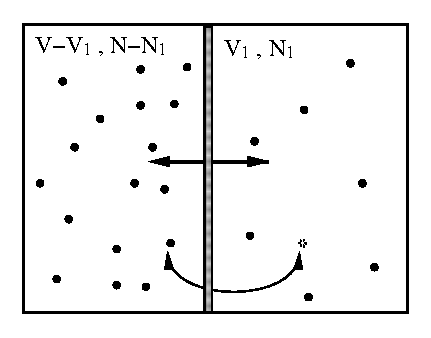
\includegraphics[width=0.5\textwidth]{Gibbs_method}
		\caption{Gibbs method scheme. From \cite{Frenkel2002}.}
		\label{fig:Gibbs_method}
	\end{figure}
	
\end{frame}


\section{Conclusions}

\begin{frame}[allowframebreaks]{Conclusions}

	Just a brief summary of what we've done.

	\begin{itemize}
		\item We've discussed the physical system studied, with a focus on how to translate the problem into something that can be handled by a machine in a ``finite'' way.
		\item We've discussed the so-called \alert{tail corrections} and we've said a lot about handling the \alert{cutoff radius} in a proper way.
		\item This was done by keeping an eye on the configuration of the system and by properly choosing the parameters of the simulation in order to get good results within the desired precision without wasting computational resources.
		\item We've briefly discussed the calculation of the uncertainties, which was done using the \alert{binning technique}.
		\item We've compared the program written for this assignment with other programs and data, highlighting many common mistakes that one could do when writing this kind of programs.
		\item In general, the program performs extremely well if compared with trustworthy data.
		\item We've then produced some data in order to show possible applications. For the isochores, we've discussed two different ways of calculating the \alert{specific heat}, highlighting the advantages of one over the other.
		\item For the isotherms we've tried to fit the data to a widely used model, in order to compare our results for the liquid-vapor \alert{coexistence curve} with the ones in the literature. We've also briefly discussed why standard NVT simulations -- as this one -- are not a good tool in the calculation of the coexistence properties.
	\end{itemize}

	\uncover<+->{Hope this was at least a little bit interesting\ldots}
	
	\begin{center}
		\Large \uncover<+->{Thanks for your attention!}
		
		\Huge\uncover<+->{\Smiley}
	\end{center}

\end{frame}

\begin{frame}[standout]
	Questions?
\end{frame}

\begin{frame}[allowframebreaks]{References}

	\nocite{*}
	\bibliographystyle{plainnat}
	\bibliography{references/ref_database}

\end{frame}

\end{document}
